%%%%%%%%%%%%%%%%%%%%%%%%%
% Dokumentinformationen %
%%%%%%%%%%%%%%%%%%%%%%%%%
\newcommand{\titleinfo}{Wechsel- \& Drehstromtechnik - HS2019}
\newcommand{\authorinfo}{Ben-Ji \& Atomjoggeli, Braun \& Co, J.Rast, S.K\"orner, C.Gwerder, M. Giger}


%% Projektheader, darf beliebig verändert werden
%Schriftgr"osse, Layout, Papierformat, Art des Dokumentes
\documentclass[10pt,a4paper,fleqn,headsepline,footsepline]{scrartcl}
%Einstellungen der Seitenränder
\usepackage[left=0.8cm,right=0.8cm,top=0.5cm,bottom=0.5cm,includeheadfoot]{geometry}
% Sprache, Zeichensatz, packages
\usepackage[UTF8]{inputenc}
\usepackage[ngerman]{babel,varioref}
\usepackage{amssymb,amsmath,graphicx,xcolor,lastpage,wrapfig,verbatim}
\usepackage{tabularx}
\usepackage{multicol}
\usepackage{rotating}
\usepackage{floatflt}
\usepackage{array}
\usepackage{scrlayer-scrpage}
\usepackage{multirow,multicol}
\usepackage{trfsigns, trsym}
\usepackage{tikz}
\usepackage{afterpage}


\usepackage[european]{circuitikz}
\usetikzlibrary{patterns}
\pgfdeclarelayer{bg}    % declare background layer
\pgfsetlayers{bg,main}
\newcommand*{\rechterWinkelRadius}{.25cm}
\newcommand*{\rechterWinkel}[2]{% #1 = point, #2 = start angle
   \draw[shift={(#2:\rechterWinkelRadius)}] (#1) arc[start angle=#2, delta angle=90, radius = \rechterWinkelRadius];
   \fill[shift={(#2+45:\rechterWinkelRadius/2)}] (#1) circle[radius=1.25\pgflinewidth];
}


\usepackage{adjustbox}
%
\setkomafont{pageheadfoot}{\footnotesize}
%
%
\RedeclareSectionCommands[
  beforeskip=-.2\baselineskip,
  afterskip=.1\baselineskip
]{section,subsection,subsubsection,paragraph}

\definecolor{pgrey}{rgb}{0.2,0.2,0.2}
\definecolor{black}{rgb}{0,0,0}
\definecolor{red}{rgb}{1,0,0}
\definecolor{white}{rgb}{1,1,1}
\definecolor{grey}{rgb}{0.8,0.8,0.8}
\definecolor{green}{rgb}{0,.8,0.05}
\definecolor{brown}{rgb}{0.603,0,0}

\DeclareMathOperator{\sinc}{sinc}
\DeclareMathOperator{\sgn}{sgn}
\DeclareMathOperator{\Real}{Re}
\DeclareMathOperator{\Imag}{Im}
%\DeclareMathOperator{\e}{e}
\DeclareMathOperator{\cov}{cov}
\DeclareMathOperator{\PolyGrad}{PolyGrad}


\newcommand{\HRule}{\noindent\rule{\linewidth}{1pt}}


\newcommand{\matlab}[1]{\footnotesize{(Matlab: \texttt{#1})}\normalsize{}}
\newcommand{\skript}[1]{${\textcolor{pgrey}{\mbox{\small{Skript S.#1}}}}$}
\newcommand{\kuchling}[1]{$_{\textcolor{red}{\mbox{\small{Kuchling #1}}}}$}
\newcommand{\stoecker}[1]{$_{\textcolor{orange}{\mbox{\small{Stöcker #1}}}}$}
\newcommand{\sachs}[1]{$_{\textcolor{blue}{\mbox{\small{Sachs S. #1}}}}$}
\newcommand{\hartl}[1]{$_{\textcolor{green}{\mbox{\small{Hartl S. #1}}}}$}

%
\newcommand{\myparagraph}[1]{\paragraph{#1}\mbox{}\\\nopagebreak}
\newcommand{\formelbuch}[1]{$\quad{\textcolor{pgrey}{\mbox{\small{S#1}}}}$}

\newcommand*{\diff}{\mathop{}\!\mathrm{d}}

\newcommand{\arraystretchOriginal}{1.5}

\newcommand{\FT}
{
\begin{picture}(1,0.5)
\put(0.2,0.1){\circle{0.14}}\put(0.27,0.1){\line(1,0){0.5}}\put(0.77,0.1){\circle*{0.14}}
\end{picture}
}

\renewcommand{\arraystretch}{\arraystretchOriginal}


\newcolumntype{L}[1]{>{\raggedright\let\newline\\\arraybackslash\hspace{0pt}}m{#1}}
\newcolumntype{C}[1]{>{\centering\let\newline\\\arraybackslash\hspace{0pt}}m{#1}}
\newcolumntype{R}[1]{>{\raggedleft\let\newline\\\arraybackslash\hspace{0pt}}m{#1}}


\author{\authorinfo}
\title{\titleinfo}
%
%Kopf- und Fusszeile
%
\lohead*{\titleinfo}
\rohead*{\today}
\lofoot*{\authorinfo}
\cofoot*{}
\rofoot*{Seite \thepage { }von \pageref{LastPage}}
%
\pagestyle{scrheadings}



% TikZ zeugs:1

\begin{document}

\section{Wechselstromtechnik}
	\subsection{Periodisch zeitabh\"angige Gr\"ossen}
 %		\subsubsection{Periodische Schwingungen}
 %			\begin{tabular}{p{6cm}p{4.5cm}p{7.5cm}}
 %				Frequenz &
 %           		\fbox{$f = \frac{1}{T} = \frac{2 \pi}{\omega}$} &
 %            		$[f] = s^{-1}$ \\ \\
 %				Schwingungsbreite &
 %					\fbox{$i_{pp} = i_{max} - i_{min}$} \\ \\
 %				Scheitelwert &
 %					\fbox{$\hat{i} = |i_{max}| \quad\text{für}\quad{|i_{max}|}\geq{|i_{min}|} \quad \text{oder} \quad \hat{i} = |i_{min}|\quad\text{für}\quad |i_{max}| < |i_{min}|$}
 %			\end{tabular}
		

		\subsubsection{Mittelwerte periodischer Gr\"ossen}
			\begin{tabular}{|p{5.5cm}|p{6cm}|p{6.5cm}|}
			\hline
				Arithmetischer Mittelwert, Gleichwert, Linearer MW &
				$X_0 = \overline{X} = X_m = \frac {1} {T} \int\limits_{t_0}^{t_0+T} x(t)dt$ &
				Ist die Fl\"ache unter der Zeitfunktion \"uber eine Periode. \\
			\hline
				MW des Quadrates, Leistung &
				$X^2 = \frac {1} {T} \int\limits_{t_0}^{t_0+T} x^2(t)dt$ & 
				$X^n = \frac {1} {T} \int\limits_{t_0}^{t_0+T} x^n(t)dt$ (MW $n$. Ordnung) \\
			\hline
				Effektivwert, Quadratischer MW &
				$X = X_{\text{eff}}= \sqrt{X^2} = \sqrt{\frac{1}{T} \int\limits ^{t_0+T} _{t_0}{x^2(t)dt}}$
				& \\ 
			\hline
				Gleichrichtwert &
				$X_{|m|} = \bar{|X|} = \frac{1}{T} \int\limits_{t_0}^{t_0+T}{|x(t)| dt}$ &
				Arithm. Mittelwert der Zweiweggleichrichterschaltung \\
			\hline				    
				Energie der Periode $T$ &
				$W_T = \int\limits_{t_0}^{t_0+T}{P(t) dt}$ &
				ist die Energie positiv, nimmt der Zweipol Energie auf \\
			\hline                    
				Wirkleistung &
				$P = \frac{1}{T} \int\limits_{t_0}^{t_0+T}{P(t) dt}  = \frac{X^2}{R}$ & \\
			\hline
			\end{tabular}
			
	\subsubsection{Verhältnisszahlen}
		\begin{multicols}{2}
			\begin{tabular}{ll}
				Scheitelfaktor $k_s$ (crest factor): 
					& $k_s = \frac{\text{Scheitelwert}} 	
							{\text{Effektivwert}} = \frac{\hat{x}}{X}$ \\
   				Formfaktor F (form factor): 
   				 	& $F = \frac{\text{Effektivwert}}
   				 			{\text{Gleichrichtwert}} = \frac{X}{|\bar{x}|}$ \\	
   				Klirrfaktor k: 
   				    & $k = \frac{\text{Effektivwert der 	
   				    					Oberwellen}}
   				    		{\text{Gesamteffektivwert}}$ \\
			\end{tabular}
			\columnbreak
	
			\begin{tabular}{ll}
				Schwingungsgehalt: 
					& $s = \frac{\text{Effektivwert des 	
										Wechselanteils}}
							{\text{Effektivwert der 		
									Mischgr\"osse}}$ \\
				Effektive Welligkeit:
					 & $\frac{\text{Effektivwert des 		
					 				Wechselanteils}}
					 		{\text{Gleichwert der 	
					 				Mischgr\"osse}}$ \\
				Riffelfaktor: 
					& $\frac{\text{Scheitelwert des 	
									Wechselanteils}}
							{\text{Gleichwert der 
									Mischgr\"osse}}$ \\
			\end{tabular}
		\end{multicols}

		\begin{tabular}{p{6.5cm}p{3cm}p{7.5cm}}
			\textbf{Simpsonsche Regel}
				&	Gleichwert: &
						$\bar{x} = \frac{\Delta t}{3T} \sum m \cdot x$ \\ 
				\textit{(Berechnungsmethode anhand}		\\
				
				\textit{eines Graphen) }
				 &	Gleichrichtwert: &
						$|\bar{x}| = \frac{\Delta t}{3T} \sum m \cdot |x|$ \\ \\
						
				 &	Effektivwert: &
						$X_{eff} = \sqrt{\frac{\Delta t}{3T} \sum m \cdot x^2}$ \\ \\
				\begin{minipage}{10cm}
					\begin{tabular}{| c | c | c | c | c | c | c | c |}
						\hline
			 				$n$ & $t$ &$x$ & $x^2$ & $m$ & $m \cdot x$ & $m \cdot x^2$ \\
			 			\hline
				 			0 & & & & 1 & & \\
				 		\hline
				 			1 & & & & 4 & & \\
				 		\hline
				 			2 & & & & 2 & & \\
				 		\hline
				 			\vdots & & & & \vdots & & \\
				 		\hline
				 			n-1 & & & & 1 & & \\
				 		\hline
			 		\end{tabular}
				\end{minipage} &
				\begin{minipage}{12.5cm}
                	\begin{itemize}
                		\item Im Graph innerhald der Periode $T$ 	
                			  eine ungerade Anzahl von $\boldsymbol{n}$ \textbf{Stützstellen} in konstanten \textbf{Abst\"anden} $\boldsymbol{\Delta t}=\frac{T}{n-1}$ w\"ahlen. Mit $t = t_0$ und $t = t_0+T$ \\ 
                			  $\rightarrow$ Zur Kontrolle $x(t_0) = x(t_0+(n-1)\cdot\Delta t)$
                		\item An diesen Stützstellen jeweils den 
                			  Augenblickswert ablesen und in die Tabelle (siehe Links) eintragen.
                		\item Anschliessend die Tabelle vervollständigen und mit den obigen Formeln summieren
                		\item \textbf{Faktor} $\boldsymbol{m}$ 
                			  wird wie folgt gebildet: Für ungerade n ist m=4; bei der ersten und bei der
                			  letzten Stützstelle ist m=1, bei den übrigen ist m=2.    
                	\end{itemize}
                \end{minipage}
			\end{tabular}
	\subsubsection{Gleichrichterschaltungen}
			\begin{tabular}{p{4cm}p{4cm}p{9cm}}
            	\begin{minipage}{4cm}
            		\textbf{Einweggleichrichtung} \\
            		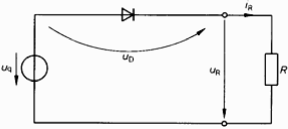
\includegraphics[height=1.2cm]{bilder/EinwegGleichrichtung.png}
            	\end{minipage} &
            		\begin{minipage}{4cm}
                    	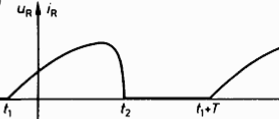
\includegraphics[width=4cm]{bilder/AusgangsspannungStromEinwegGleichrichtung.png}
                    \end{minipage} &
					\begin{minipage}{8cm}
                    	Fliesst nur ein Strom in Durchlassrichtung der Diode. \\
                    	Summe der Oberwellen $i_0=0.2176A$ \\
                    	$t_1 < t < t_2$ $\Rightarrow$ $u_R = u_q$ ; $i_R = u_q/R$ ; $u_D = 0$ \\
                    	$t_2 < t < (t_1+T)$ $\Rightarrow$ $u_R = 0$ ; $i_R = 0$ ; $u_D = u_q$
                    \end{minipage} \\
				\begin{minipage}{4cm}
                	\textbf{Zweiweggleichrichtung} \\
                	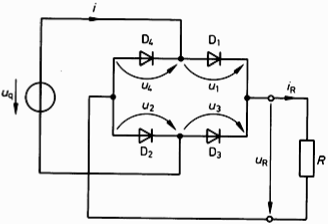
\includegraphics[height=1.5cm]{bilder/BrueckenGleichrichtung.png}
                \end{minipage} &
					\begin{minipage}{4cm}
                    	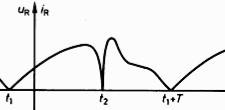
\includegraphics[width=4cm]{bilder/AusgangsspannungBrueckenGleichrichtung.png}
                    \end{minipage} &
					\begin{minipage}{9cm}
                    	Ausgangsspannung ist Betrag der Eingangsspannung. \\
                    	$t_1 < t < t_2$ $\Rightarrow$ $D_1,D_2$ leiten ; $D_3,D_4$ sperren \\
                    	$t_2 < t < (t_1+T)$ $\Rightarrow$ $D_1,D_2$ sperren ; $D_3,D_4$ leiten \\
                    	$u_R = |u_q|$ ; $i_R = u_R/R = |i|$
                    \end{minipage}
            \end{tabular}
	\subsection{Sinusf\"ormige Schwingungen von Spannung und Strom}
 		\subsubsection{Erzeugung sinusf\"ormiger Schwingungen}
 			\begin{minipage}{6cm}
 				\textbf{Lenzsche Regel}\\
 					Der induzierte Strom wirkt seiner Ursache entgegen.\\
 					Ursache des induzierten Stromes ist die \"Anderung des Flusses.
             \end{minipage}
             \hfill
 			\begin{minipage}{4.5cm}
 				\textbf{Bewegte Leiter im \\ homogenen Magnetfeld}\\
             	$U = B \cdot l \cdot v_q$ \\
             	             	$v_q = v \cdot cos\beta = v \cdot sin\alpha\\$
             	$U = \hat{U} \cdot sin \alpha$
             \end{minipage}
 			\begin{minipage}{3.5cm}
             	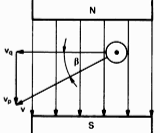
\includegraphics[width=3.5cm]{bilder/BewegteLeiter.png}
             \end{minipage}
 			\begin{minipage}{3.5cm}
             	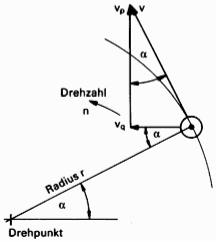
\includegraphics[width=3.5cm]{bilder/KreisfoermigeBewegung.png}
             \end{minipage}
% 		\subsubsection{Beschreibung sinusf\"ormiger Spannungen und Str\"ome}
% 			\begin{tabular}{p{6cm}p{4.5cm}p{7.5cm}}
%             	\textbf{Kreisfrequenz} &
%             		\fbox{$\omega = \frac{2 \pi}{T} = 2 \pi f$} &
%             		$[\omega] = s^{-1}$ \\ \\
%             	\textbf{Effektivwert für sinusf\"ormige Gr\"ossen} &
%             		\fbox{$U = \frac{\hat{u}}{\sqrt{2}} \quad I = \frac{\hat{i}}{\sqrt{2}}$}
%             \end{tabular}
		\subsubsection{Komplexe Zeiger}
			\begin{minipage}[t]{6cm}
            	\textbf{Prinzip der Zeigertechnik}
            \end{minipage}
			\begin{minipage}{6cm}
            	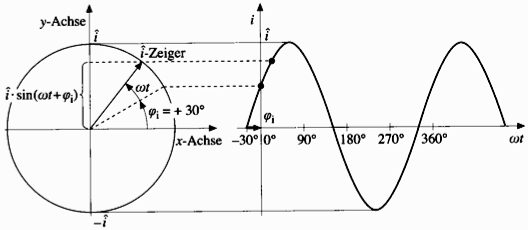
\includegraphics[width=6cm]{bilder/RotierenderScheitelwertzeiger.png}
            \end{minipage}
			\begin{minipage}{3.5cm}
            	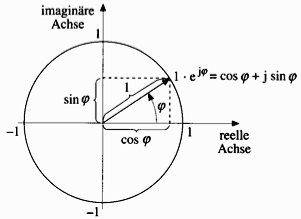
\includegraphics[width=3.5cm]{bilder/EulerscheRelation.png}
            \end{minipage} \\
			\begin{tabular}{p{4.0cm}p{5.5cm}p{8.5cm}}
            	Komplexer Effektivwert &
            		$\underline{U} = \frac{\underline{\hat{u}}}{\sqrt{2}}$ &
            		$\underline{U}$ = Kompl. Effektivwert, $\underline{\hat{u}}$ = Kompl. Scheitelwert \\
				Exponentialform &
					$\underline{\hat{u}} = \hat{u} \cdot e^{j\varphi_u} \quad \underline{U} = U \cdot e^{j\varphi_U}$  &
					$\varphi_U$ = Nullphasenwinkel der Spannung\\
				Algebraische Form &
					$\underline{\hat{u}} = \hat{u} (\cos(\varphi_u)+j\sin(\varphi_u))$ &
					$\Real(\underline{\hat{u}}) = \hat{u} \cdot \cos(\varphi_u)$ \quad $\Imag(\underline{\hat{u}}) = \hat{u} \cdot \sin(\varphi_u)$ \\
				&	$\underline{U} = U (\cos(\varphi_U)+j\sin(\varphi_U))$ &
					$\Real(\underline{U}) = U \cdot \cos(\varphi_U)$ \quad $\Imag(\underline{U}) = U \cdot \sin(\varphi_U)$ \\
				Umrechnung &
					$|\hat{u}| = \sqrt{\Real(\underline{\hat{u}})^2 + \Imag(\underline{\hat{u}})^2}$ \break $\varphi_u = \arctan\left(\dfrac{\Imag(\underline{\hat{u}})}{\Real(\underline{\hat{u}})}\right)$ \\
				&	$|U| = \sqrt{\Real(\underline{U})^2 + 		\Imag(\underline{U})^2}$ \break
					 $\varphi_u = \arctan\left(\dfrac{\Imag(\underline{U})}{\Real(\underline{U})}\right)$ \\
				Komplexe Drehzeiger & 	
					\multicolumn{2}{l}{$\underline{u}(t) = \underline{\hat{u}} \cdot e^{j\omega t} = \hat{u} \cdot e^{j\varphi_u} \cdot e^{j\omega t} = \hat{u} \cdot e^{j(\omega t + \varphi_u})$} \\
				Phasenwinkel & 
					$\varphi = \varphi_u - \varphi_i$ &
					$\varphi > 0$: $U$ eilt $I$ vor\\ 
				& 	$\varphi = \frac{\Delta t}{T}\cdot 2\pi$ &
					$\varphi < 0$: $U$ eilt $I$ nach\\
			\end{tabular}
		\subsubsection{Komponenten linearer Wechselstromnetzwerke}% \formelbuch{125}}
			\begin{tabular}{llll}
			$\underline{Z} = R +j X$: 
				& Komplexer Widerstand (Impedanz); 
				& $R$: Wirkwiderstand (Resistanz); 
				& $X$: Blindwiderstand (Reaktanz)\\
			$\underline{Y} = G + j B$: 
				& Komplexer Leitwert (Admittanz); 
				& $G$: Wirkleitwert (Konduktanz); 
				& $B$: Blindleitwert (Suszeptanz)
	      	\end{tabular} \\ \\
			\begin{tabular}{|l|l|l|l|l|l|ll|}
			\hline
				\textbf{Widerstand} & 
					\multicolumn{2}{l|}{$ \underline{Z}_R = R$} & \multicolumn{2}{l|}{$ \underline{Y}_R = G =\frac{1}{R}$} &
					&
					\parbox[c][0.8cm][c]{1cm}{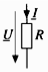
\includegraphics[height=1cm,angle=90]{bilder/Wirkwiderstand.png}}&
                	\parbox[c][0.8cm][c]{1cm}{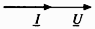
\includegraphics[width=1cm]{bilder/WirkwiderstandZeiger.png}} \\
			\hline	                    
				\textbf{Induktivit\"at} &
					$ \underline{Z}_L = j \omega L = j X_L$&
					$ X_L = \omega L$ &
					$ \underline{Y}_L = \frac{1}{j \omega L} = j B_L$ & 
					$ B_L = - \frac{1}{\omega L}$ &
					$ W_L=\frac12 L {I_L}^2$  &
					
		            \parbox[c][0.8cm][c]{1cm}{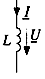
\includegraphics[height=1cm,angle=90]{bilder/Spule.png}}&
		            \parbox[c][1cm][c]{1cm}{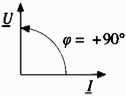
\includegraphics[width=1cm]{bilder/SpuleZeiger.png}}
		            \\
			\hline		                
				\textbf{Kondensator} &
					$ \underline{Z}_C = \frac{1}{j \omega C} = jX_C $ &
					$ X_C = - \frac{1}{\omega C} $ &
					$ \underline{Y}_C = j \omega C = j B_C $&
					$ B_C = \omega C $ &
					$ W_C=\frac12 C {U_C}^2$ & 
		            \parbox[c][0.8cm][c]{0.8cm}{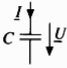
\includegraphics[height=0.9cm,angle=90]{bilder/Kondensator.png}}&
		            \parbox[c][1cm][c]{1cm}{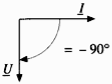
\includegraphics[width=1cm]{bilder/KondensatorZeiger.png}}\\
			\hline	    
				\parbox[c][1cm][c]{2cm}{}&
					\multicolumn{2}{l|}
						{$ \underline{Z} = \frac{\underline{U}}{\underline{I}} = \frac{\underline{U}^2}{\underline{S}^*} = 
							\frac{\underline{S}}{\underline{I}^2} $} &
					\multicolumn{2}{l|}
					{$ \underline{Y} = \frac{\underline{I}}{\underline{U}} = \frac{1}{\underline{Z}} $} &
					&
					& \\
			\hline       
			\end{tabular}
	%	\subsubsection{Berechnung linearer Wechselstromnetzwerke}
		\renewcommand{\arraystretch}{2}
		\subsubsection{Leistung im Wechselstromnetzwerk}% \formelbuch{162}}
				\begin{tabular}{p{4cm}p{7cm}p{7cm}}
					\multirow{2}{4cm}{Komplexe Leistung}  &
						$ \underline{S} = P + jQ$  &\\
						& $ \underline{S} = \underline{U} \cdot \underline{I}^\ast = U\cdot I \cdot e^{j(\varphi_u-\varphi_i)} = \frac{\underline{U}^2}{\underline{Z}^*} = \underline{I}^2 \cdot \underline{Z}$ &
						\\
					Scheinleistung [VA]	& $ S = U\cdot I = \frac{U^2}{Z} 
						= I^2 \cdot Z = \sqrt{P^2+Q^2}$& \\
					Wirkleistung [W] &
						$ P = \Real(\underline{S}) = S \cos(\varphi) = I^2 \cdot \Real(\underline{Z}) $ \\
					Blindleistung [var] &
						$ Q = \Imag(\underline{S}) = S \sin(\varphi)  = P \cdot
						\tan\left(\varphi\right)$ & Kapazitiv: $Q < 0$; induktiv: $Q > 0$ \\
					Leistungsfaktor &
						$\lambda = \frac{P}{S} = \frac{P}{U\cdot I} = \underbrace{\cos \varphi}_{\text{bei sinus Schwingungen}}$ \\
				\end{tabular}
		\renewcommand{\arraystretch}{1}
		\subsubsection{Blindleistungskompensation (mit Kondensator)}
		\renewcommand{\arraystretch}{1.5}
\begin{tabular}{p{7cm}p{4.5cm}p{5cm}}
	Kompensation mit C &
    	\begin{minipage}{4cm}
        	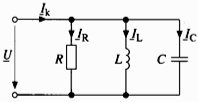
\includegraphics[width=3.5cm]{bilder/Parallelkompensation.png}
        \end{minipage} & 
		Der Kondensator wird parallel dazu geschalten \\ \\
	Zeigerdiagramme Kompensation &
		\begin{minipage}{4.5cm}
        	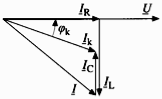
\includegraphics[width=3.5cm]{bilder/Blindstromkompensation.png}
        \end{minipage} &
		\begin{minipage}{4.5cm}
        	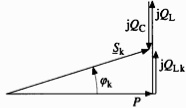
\includegraphics[width=3.5cm]{bilder/Blindleistungskompensation.png}
        \end{minipage} \\ \\
	Neue (kompensierte) Blindleistung &
		$Q_{Lk} = P \cdot \tan{\varphi_k}$ \\
	Blindleistung des Kondensators & 
		\multicolumn{2}{l}{$Q_C = Q_{Lk} - Q_L =  P\cdot (\tan{\varphi_k}-\tan{\varphi}) $} \\
	Kapazität des Kondensators &
		$C = - \frac{Q_C}{\omega U^2}$ \\	
	\end{tabular}
\renewcommand{\arraystretch}{1}
		\begin{multicols}{2}
			\subsubsection{Serieschaltung von $R_S$ \& $X_S$}
				\begin{tabular}{lll}
			%		& $Z = R_S + jX_S$ &\\
			%		& $\varphi = \arctan(\frac{X_S}{R_S})$ & \\
			%		& $U_R = U_0 \cdot \cos\varphi $& \\
			%		& $U_X = U_0 \cdot \sin\varphi $ & \\
			%		& $P = \frac{U_R^2}{R_S} = I^2\cdot R_S$ &\\
			%		& $Q = \frac{U_X^2}{X_S} = I^2\cdot X_S$&
				\end{tabular}
				\begin{align*} 
					Z 		&	= R_S + jX_S 				  \\
					\varphi &	= \arctan(\frac{X_S}{R_S}) 	  \\
					U_R 	&	= U_0 \cdot \cos\varphi 	  \\
					U_X		&	= U_0 \cdot \sin\varphi 	  \\
					P		&	= \frac{{U_R}^2}{R_S} = {I_0}^2\cdot R_S  \\
					Q		&	= \frac{{U_X}^2}{X_S} = {I_0}^2\cdot X_S					
				 \end{align*}
			\columnbreak 
			\subsubsection{Parallelschaltung von $R_P$ \& $X_P$}
				\begin{align*}
					Z 		&	= \frac{1}{\frac{1}{R_P}+j(-\frac{1}{X_P})}	\\
					\varphi &	= \arctan(- \frac{R_P}{X_P})				\\
					I_R 	&	= I_0 \cdot \cos\varphi						\\
					I_X		&	= I_0 \cdot \sin\varphi						\\
					P		&	= \frac{{U_0}^2}{R_P} = {I_R}^2\cdot R_P	    \\
					Q		&	= \frac{{U_0}^2}{X_P} = {I_X}^2\cdot X_P
				\end{align*}
		\end{multicols}

		\subsubsection{Leistungsumsatz bei nichtsinusf\"ormigen periodischen Gr\"ossen}
		\begin{minipage}[c]{7.5cm}
			\parbox{4cm}{Allgemein: Indizes beziehen sich auf Harmonische (Bsp: 0. Har = DC)\\}
			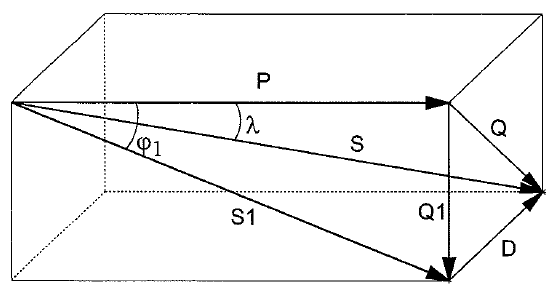
\includegraphics[height=4cm]{bilder/ZeigerdiagrammNichtSinus.png}     
    	\end{minipage}
		\begin{minipage}[c]{10.5cm}   
    		\noindent
    		\renewcommand{\arraystretch}{2.5}
    		\begin{tabular}{p{1.8cm} p{5.6cm}}
        		Unterwelle: 
        			& $X_{U} = \overline{X} = \dfrac{\hat{X}}{\sqrt{2}} a_0 \qquad $  \\
	     		Grundwelle: 
	     			& $X_{G} = \dfrac{\hat{X}}{\sqrt{2}} \sqrt{a_1^2 + b_1^2} \qquad  $   \\
	     		Oberwellen: 
	     			& $X_{O} = \dfrac{\hat{X}}{\sqrt{2}}
	     			\sqrt{\sum\limits_{k=2}^{\infty}a_k^2 +\sum\limits_{k=2}^{\infty}b_k^2}
	     			\qquad $  \\ 
	     		\multicolumn{2}{l}{Effektivwerte: $X_{RMS} = \sqrt{X_G^2 + X_O^2} \qquad X_{TRMS} =
	     			\sqrt{X_U^2 + X_{RMS}^2}$ } \\
				\multicolumn{2}{l}{ges. Blindleistung: 
					$Q = 	\sqrt{Q_G^2 + Q_U^2 + U^2 \sum\limits_{k=2}^{\infty}I_k^2} = \sqrt{U^2 \sum\limits_{k=0}^{\infty}I_k^2}$} \\ 
				\multicolumn{2}{l}{Grundschwinungs-Blindleistung: 
					$Q_1 = \sqrt{{S_1}^2 - P^2}$} \\
				\multicolumn{2}{l}{Wirkleistung: 
					Durch Signale gleicher Frequenz umgesetzt, $P_R = {I_{TRMS}}^2 \cdot R$} \\
				\multicolumn{2}{l}{Verzerrungsblindleistung: 
					$D = U \cdot \sqrt{I_0^2 + \sum\limits_{k=2}^{\infty}I_k^2}$} \\
				\multicolumn{2}{l}{Grundschwinungs-Scheinleistung: 
					$S_1 = U \cdot I_G$} \\
				\multicolumn{2}{l}{ges. Scheinleistung: 
					$S = \sqrt{P^2 + {Q_1}^2 + D^2} = U \cdot I_{TRMS}$} \\
		 	\end{tabular} \\
		 \renewcommand{\arraystretch}{1}
     	\end{minipage}    		\\ \\
     	Die Verzerrungsblindleistung wird von den Oberwellen und ev. von der Unterwelle (je
     	nach Phasenverschiebung) verursacht und ist mit Kondensatoren \textbf{nicht} zu kompensieren -
     	Aktive Filter w\"aren n\"otig.
		\\		
		
	\begin{minipage}[c]{8cm} 
	   \textbf{Beispiel anhand eines Einweggleichrichters:}	  	\\
	   (mit ohmscher Last R) 
	\end{minipage}   
	\begin{minipage}[c]{10cm} 	
	   $ \qquad i(t) = \underbrace{\frac{\hat{I}}{\pi}}_{Unterwelle} + \underbrace{\frac{\hat{I}}{2}
	   \sin(\omega t)}_{Grundwelle} - \underbrace{\frac{2\hat{I}}{\pi} \sum\limits_{k=1}^n \frac{1}{(2k-1)(2k+1)} \cos(2k\omega t)}_{Oberwellen} $
	\end{minipage}   
		
	\begin{minipage}[c]{10cm}  
		\begin{tabular}{| l | l |}
    		\hline 
      		\textbf{Bezeichnung}
      		%& \textbf{N\"aherungsformel}
      		& \textbf{Formel} \\
      		\hline
      		Scheitelwert 
      		%& %& $\hat{I} = 0.7071 \cdot A $
      		& $\hat{I} = \hat{I}_d = \frac{\hat{U}_d}{R} $ \\
      		Unterwelle (Mittelwert)
      		%& $I_U = 0.22508 \cdot A $
      		& $I_U = I_m = \bar{I}_d  = \frac{\hat{I}}{\pi}$ \\
      		Grundwelle
      		%& $I_G = 0.25 \cdot A$ 
      		& $I_G = \frac{\hat{I}}{2 \cdot \sqrt{2}}$ \\
      		Oberwelle
      		%& $I_O = 0.10881 \cdot A$ 
      		& $I_O = \frac{\hat{I}}{\sqrt{2}} \cdot 0.21762$ \\
      		%Effektivwert (RMS)
      		%& $I_{RMS} = 0.27265 \cdot A$
      		%& $I_{RMS} = \sqrt{I_G^2 + I_O^2}$ \\
      		Laststrom
      		%& $I_{TRMS} = 0.35355 \cdot A$
      		& $I_{d} = I_{TRMS} =\frac{\hat{I}_d}{2} = \frac{U_d}{R}$ \\
      		Prim\"arstrom
      		& $I_1 \approx \bar{I}_d \cdot \frac{1.21}{"u}$ \\
      		Leistungen
      		& $Q = D | S_1 = P | Q_1 = 0$ \\
      		%Bauleistung 
      		%& $S_{TR} = \frac{S_{1Tr} + S_{2Tr}}{2}$ \\
      		\hline 
    	\end{tabular}
	\end{minipage}   
	\begin{minipage}[c]{8cm}  
			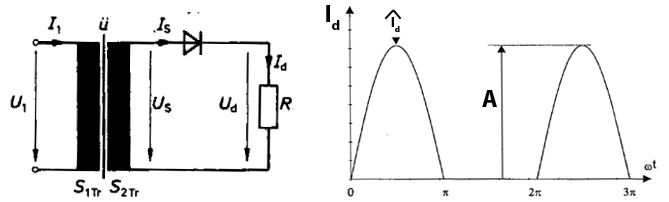
\includegraphics[width=8cm]{bilder/EinwegGR.png}  \\			
	$S_{1Tr} < S_{2Tr}$ da der Trafo keine Gleichstr\"ome übertr\"agt. Somit erscheint der Prim\"arstrom
	als Sekund\"arstrom mit unterdrücktem Gleichstromanteil.\\			
	\end{minipage}

	\begin{minipage}[c]{8cm} 
	   \textbf{Beispiel anhand eines Brückengleichrichters:}	  	\\
	   (mit ohmscher Last R)
	\end{minipage}   
	\begin{minipage}[c]{10cm} 	
	   $ \qquad i(t) = \underbrace{\frac{2 \hat{I}}{\pi}}_{Unterwelle} - \underbrace{\frac{4\hat{I}}{\pi} \sum\limits_{k=1}^n \frac{1}{(2k-1)(2k+1)} \cos(2k\omega t)}_{Oberwellen} $
	\end{minipage}\\
\begin{minipage}[c]{10cm}  
		\begin{tabular}{| l | l |}
    		\hline 
      		\textbf{Bezeichnung}
      		%& \textbf{N\"aherungsformel}
      		& \textbf{Formel} \\
      		\hline
      		Scheitelwert 
      		%& %& $\hat{I} = 0.7071 \cdot A $
      		& $\hat{I} = \hat{I}_d = \frac{\hat{U}_d}{R} $ \\
   %   		Fourien-Reihe
    %  		&$i(t)=A(\frac{2}{\pi}-\frac{4}{\pi}(\frac{\cos(2t)}{1\cdot
 %     		3}+\ldots+\frac{\cos(2nt)}{(2n-1) \cdot (2n+1)}))$\\
      		Unterwelle (Mittelwert)
      		%& $I_U = 0.22508 \cdot A $
      		& $I_U = \bar{I}_d = \frac{2 \hat{I}}{\pi}$ \\
      		Grundwelle
      		%& $I_G = 0.25 \cdot A$ 
      		& $I_G = 0$ \\
      		Oberwelle
      		%& $I_O = 0.10881 \cdot A$ 
      		& $I_O = \frac{\hat{I}}{\sqrt{2}} \cdot 0.43524$ \\
      		%Effektivwert (RMS)
      		%& $I_{RMS} = 0.27265 \cdot A$
      		%& $I_{RMS} = \sqrt{I_G^2 + I_O^2}$ \\ 
      		Laststrom
      		%& $I_{TRMS} = 0.35355 \cdot A$
      		& $I_{d} = I_{TRMS} =  \frac{U_s}{R}= \frac{\hat{U}_d}{\sqrt{2}R}$ \\ 
      		Diodenstrom
      		& $I_{V} = \frac{\hat{U}}{2 R} = \frac{I_{d}}{\sqrt{2}}$ \\
      		Prim\"arstrom
      		& $I_1 \approx \bar{I}_d \cdot \frac{0.966}{"u}$ \\
      	%	Bauleistung 
      	%	& $S_{TR} = \frac{S_{1Tr} + S_{2Tr}}{2}$ \\
      	 	\hline
    	\end{tabular}
	\end{minipage}   
	\begin{minipage}[c]{8cm}  
			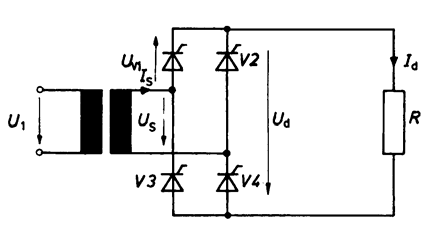
\includegraphics[width=7cm]{bilder/brueckengleichrichter.png}  \\			
	$S_{1Tr} < S_{2Tr}$ da der Trafo keine Gleichstr\"ome übertr\"agt. Somit erscheint der Prim\"arstrom
	als Sekund\"arstrom mit unterdrücktem Gleichstromanteil.			
	\end{minipage}

\section{Transformator}
		
	\subsection{Trafomodelle}
%		\subsubsection{Grundstrucktur des Trafo}
%			\begin{tabular}{p{7cm}p{4.5cm}p{5cm}}
%	        	\textbf{} &
%	        		\begin{minipage}{4.5cm}
%		            	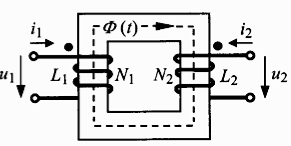
\includegraphics[width=3.5cm]{bilder/GrundstruckturTrafo.png}
%		            \end{minipage} \\
%	        \end{tabular}
		\subsubsection{Der ideale Trafo}
			\begin{tabular}{p{7cm}p{4.5cm}p{5cm}}
				Übersetzungsverh\"altnis &
					$\text{ü} = \frac{|\underline{U}_1|}{|\underline{U}_2|} =
					\frac{|\underline{I}_2|}{|\underline{I}_1|} = \frac{N_1}{N_2}$ &
					\begin{minipage}{4.5cm}
						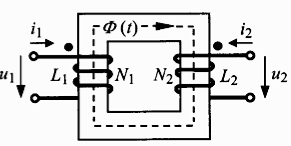
\includegraphics[width=3.5cm]{bilder/GrundstruckturTrafo.png}
					\end{minipage} \\
				Leistungsbilanz &
					$\underline{S}_1 = \underline{S}_2$ &
					oder $\underline{U}_2 \cdot \underline{I}_2^* = \underline{U}_1 \cdot \underline{I}_1^*$ \\
				Scheinwiderstandsübersetztung &
					$\underline{Z}_{aU} = \frac{|\underline{U}_1|^2}{|\underline{U}_2|^2} \cdot \underline{Z}_a = \text{ü}^2 \cdot \underline{Z}_a$ &
					\begin{minipage}{4.5cm}
	            		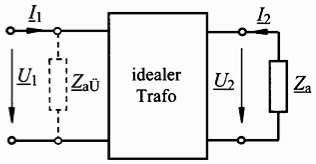
\includegraphics[width=3.5cm]{bilder/IdealerTravoImpedanzwandler.png}
	            	\end{minipage}
			\end{tabular}
		%TODO: 02.02.12 DK, Newpage wieder entfernen wen möglich 
		\newpage
		
		\subsubsection{Verlustloser und Streuungsfreier Trafo}
			\renewcommand{\arraystretch}{1.5}
\textbf{Induktionsgesetz}\\
		\begin{tabular}[c]{p{8.7cm}}
			$u_i= \mp \dot{\Phi} = \mp \frac{d}{dt} \int \vec{B} \cdot
			\vec{dA}\qquad $ \parbox{3cm}{\tiny{$- \Rightarrow B,u_i $
			Rechtsschraube\\ $+ \Rightarrow B,u_i $
			Linksschraube}}
			\\
			
			$u_i= \mp \dot{\Psi}\qquad$ , meist $\; u_i = \mp
			N\cdot\dot{\Phi}$		
		\end{tabular}
		\parbox{8cm}{Durchsetzt das sich \"andernde Magnetfeld einer stromdurchflossenen Spule
					eine zweite Spule, so wird auch in dieser eine Spannung
					(=Gegeninduktionsspannung) induziert.}	

\begin{multicols}{2}
 		\textbf{Gegeninduktion} ($M_{\textcolor{red}{X}\textcolor{green}{Y}}; \textcolor{red}{X}$: Wirkung,
 		$\textcolor{green}{Y}$: Ursache)\\
		\begin{tabular}{ll}
  		Gegeninduktivit\"at
  			& $M_{21} = \frac{\Psi_{m21}}{i_1}$ Meist $= \frac{N_2 \phi_{m21}}{i_1}$\\ 
  			(wenn $\mu$ = const.) & $M = k \cdot \sqrt{L_1 L_2} = M_{21} = M_{12} $  \\
  			Gegeninduktionsspannung
  			& $u_{21} = \dot{\Psi}_{21} = M_{21} \frac{di_1}{dt}$ \\
		\end{tabular}\\

  		\textbf{Transformatorgleichungen}\\
		$\boxed{u_1 = L_1 \dfrac{di_1}{dt} \textcolor{red}{+}\textcolor{green}{-}M_{12}
		\dfrac{di_2}{dt} = L_1 \dfrac{di_1}{dt} \textcolor{red}{-}\textcolor{green}{+}M_{12} \dfrac{di_b}{dt}}$ \\
		$\boxed{u_2 = L_2 \dfrac{di_2}{dt}\textcolor{red}{+}\textcolor{green}{-} M_{21}
		\dfrac{d i_1}{dt} = -L_2 \dfrac{di_b}{dt}
		\textcolor{red}{+}\textcolor{green}{-} M_{21} \dfrac{d i_1}{dt}}$\\
		Im Bildbereich:\\
		$\underline{U}_1 = j\omega\cdot L_1 \cdot \underline{I}_1 + j\omega\cdot M \cdot \underline{I}_2$\\
		$\underline{U}_2 = j\omega\cdot L_2 \cdot \underline{I}_2 + j\omega\cdot M \cdot \underline{I}_1$\\
  			
	  	\textbf{Idealer Trafo}\\ 
	  	$"u = \dfrac{u_1}{u_2} = \dfrac{N_1}{N_2} = \sqrt{\dfrac{L_1}{L_2}}$ $\qquad$ (im Leerlauf:
	  	$\dfrac{1}{"u} = k \sqrt{\dfrac{L_2}{L_1}}$)\\

  		\textbf{Verlustbehafteter Trafo}
  		\begin{list}{$\bullet$}{\setlength{\itemsep}{0cm} \setlength{\parsep}{0cm} \setlength{\topsep}{0cm}} 
          \item Prim\"arstrom im Leerlauf: $L_H$
          	(ideal $L_H \rightarrow \infty)$
          \item Hysterese- \& Wirbelstromverluste: $R_{Fe}$ \newline
          	(ideal: $R_{Fe}\rightarrow \infty$) 
          \item Kupferwiderst\"ande: $R_{Cu1}, R_{Cu2}$
          	(ideal: $R_{Cu}
          \rightarrow 0$)
          \item Streufluss (Kopplung): $L_{\sigma1}, L_{\sigma2}$
          	(ideal: $L_{\sigma} \rightarrow 0$)
        \end{list}

	\columnbreak
  		\begin{flushleft}
  		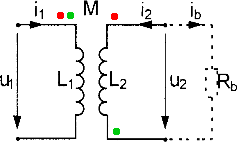
\includegraphics[width=4cm]{bilder/trafo-kopplung.png} \\
  		\small{\textcolor{red}{Gleichsinnig} / \textcolor{green}{Gegensinnig}} \\
  		\vspace{1cm}

	  	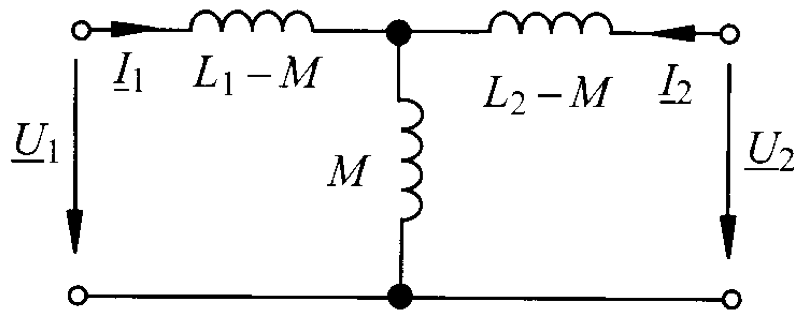
\includegraphics[width=5cm]{bilder/T_Ersatzschaltbild_VST.png}\\
		\end{flushleft}  	
	
\end{multicols}
\renewcommand{\arraystretch}{1} 	
		\subsubsection{Transformatoren-Hauptgleichung (gilt bei Leerlauf)}
			\begin{tabular}{p{7cm}p{4.5cm}p{5cm}}
      			$| \hat{u}_{10} | = \hat{i}_0 \cdot X_{L1}$
      			& 	$\hat{u}_{10} = \hat{i}_0 \cdot \omega \cdot L_1$ \\
      		
				$U_{20} = \frac{2\pi}{\sqrt{2}}N_2 f \hat{B}_1 A$
				&
            	$U_{10} = \frac{2\pi}{\sqrt{2}}N_1 f \hat{B}_1 A$ &
					wobei $\frac{2\pi}{\sqrt{2}} = 4.44$ und $\hat{B} \cdot A = \hat{\Phi}$ 
			\end{tabular}
	\subsection{Der reale (einphasige) Transformator}
		Für dreiphasige Trafos müssen die angegebenen Werte zuerst normiert werden (siehe Kapitel 3).
		\subsubsection{Ersetzen der magnetischen Kopplung}
			\begin{tabular}{p{5.8cm}p{7.3cm}p{4.5cm}}
            	Spannung, Strom &
            		$U_2' = U_2 \cdot \frac{N_1}{N_2}$ \quad 
            		$I_2' = I_2 \cdot \frac{N_2}{N_1}$ \\
            	Nennstrom & 
            		$I_N = S_N / U_N$
            	Widerstand, Streufluss &
            		$R_2' = R_2 \cdot (\frac{N_1}{N_2})^2$ \quad 
            		$X_{\sigma 2}' = X_{\sigma 2} \cdot (\frac{N_1}{N_2})^2$ \\
            	Vollst\"andiges Ersatzschaltbild &
            	\adjustbox{width=6cm}{\begin{circuitikz}[european]
	\draw (0,0) coordinate (In1) {} 
		to[short, *-, i=$\underline{I_1}$] ++(1,0)
		to[R, l=$R_1$] ++(2,0)
		to[L, l=$jX_{\sigma 1}$] ++(2,0)
		to[short, -*] ++(1,0) coordinate (middle1) {}
		to[short] ++(1,0)
		to[L, l=$jX'_{\sigma 2}$] ++(2,0)
		to[R, l=$R'_2$] ++(2,0)
		to[short, -* ,i<=$\underline{I_2}$] ++(1,0) coordinate(Out1);
	\draw (middle1) to[short, -*] ++(0,-1) coordinate (middle2) {};
	\draw (middle2) -- ++(-1,0) 
		to[R, l=$R_{Fe}$] ++(0,-2)
		to[short, -*] ++(1,0) coordinate(middle3)
		to[short, -*] ++(0,-1) coordinate(middle4);
	\draw (middle2) -- ++(1,0)
		to[L, l=$jX_h$] ++(0,-2)
		to[short] (middle3);
	\draw (middle4) to[short, -*] ++(-6,0) coordinate(In2);
	\draw (middle4) to[short, -*] ++(6,0) coordinate(Out2);
	\begin{scope}[
		shorten <=10pt,
		shorten >= 10pt,
		->
	]
		\draw (In1) -- (In2) node[midway, right] {$\underline{U_1}$};
		\draw (Out1) -- (Out2) node[midway, left] {$\underline{U'_2}$};
	\end{scope}
\end{circuitikz}}
            	&
					\begin{minipage}{4.5cm}
                    	\tiny
                    		$R_1, R_2'$: Widerstand Spule\\ \\
                    		$jX_{\sigma 1}, jX_{\sigma 2}'$: Streufluss Spule\\ \\
                    		$R_{Fe}$: Eisenverlust\\ \\
                    		$jX_h$: Hauptfluss Spule\\
                    \end{minipage} \\ \\
				Systemgleichung des realen Trafo &
					$\underline{U}_1 = R_1\cdot\underline{I}_1 + jX_{\sigma 1}\cdot\underline{I}_1 + jX_h\cdot(\underline{I}_1+\underline{I}_2')$ \\
					& $\underline{U}_2' = R_2'\cdot\underline{I}_2' + jX_{\sigma 2}'\cdot\underline{I}_2' + jX_h\cdot(\underline{I}_1+\underline{I}_2')$

            \end{tabular}
            
            	Für mittlere Transformatorenleistungen erbgeben sich etwa folgende Relationen zwischen
            	den einzelnen $R$s und $X$s:
            	$$ R_1 : R_2' : X_{\sigma 1} : X_{\sigma 2}' : X_h : R_{Fe} \approx 1:1:2:2:1000:10000	$$
            	
		\subsubsection{Leerlauf und Magnetisierung}
			\begin{tabular}{p{5cm}p{6cm}p{7cm}}
            	Rechnen &
            		\begin{minipage}{13cm}
                    	Mit Leerlaufdaten $R_{Fe}$ und $X_h$ ausrechnen. $R_1$ und $X_{\sigma1}$ vernachl\"assigen.
                    \end{minipage} \\ \\
            	Induktiver Leerlaufstrom &
            		$\underline{I}_{10} = \underline{I}_{1Fe} + \underline{I}_{1\mu}$ $(\underline{I}_{1\mu} \gg \underline{I}_{1Fe})$ &
            		\begin{minipage}{8cm}
	            		\adjustbox{width=6cm}{\begin{circuitikz}[european]
	\draw (0,0) coordinate (In1) {} 
		to[short, *-, i=$\underline{I}_{10}$] ++(1,0)
		to[R, l=$R_1$] ++(2,0)
		to[L, l=$jX_{\sigma 1}$] ++(2,0)
		to[short, -*] ++(1,0) coordinate (middle1) {}
		to[short, -* ,i<=\mbox{$\underline{I}_2 = 0$}] ++(3,0) coordinate(Out1);
	\draw (middle1) to[short, -*] ++(0,-1) coordinate (middle2) {};
	\draw (middle2) 
		to[short, i_=$\underline{I}_{1Fe}$] ++(-1,0) 
		to[R, l=$R_{Fe}$] ++(0,-2)
		to[short, -*] ++(1,0) coordinate(middle3)
		to[short, -*] ++(0,-1) coordinate(middle4);
	\draw (middle2) 
		to[short, i=$\underline{I}_{1\mu}$] ++(1,0)
		to[L, l=$jX_h$] ++(0,-2)
		to[short] (middle3);
	\draw (middle4) to[short, -*] ++(-6,0) coordinate(In2);
	\draw (middle4) to[short, -*] ++(3,0) coordinate(Out2);
	\begin{scope}[
		shorten <=10pt,
		shorten >= 10pt,
		->
	]
		\draw (In1) -- (In2) node[midway, right] {$\underline{U}_{10}$};
		\draw (Out1) -- (Out2) node[midway, right] {$\underline{U}'_{20}$};
	\end{scope}
\end{circuitikz}}
	            	\end{minipage} \\ \\
				Magnetisierungsstrom &
					$i_\mu = \sqrt{2}I_{\mu1}\cdot \sin(\omega t) + \sqrt{2}I_{\mu3}\cdot \sin(3\omega t) + \sqrt{2}I_{\mu m}\cdot \sin(m\omega t)$ &
					\hspace{3.3cm}$(m=2n+1 \hspace{0.3cm} n\epsilon \mathbb{N}_0)$ \\
					&
					Für den Effektivwert des Stromes: &
					$I_{\mu RMS} = \sqrt{I_{\mu1}^2 + I_{\mu3}^2 +\ldots+ I_{\mu m}} $\\ \\
				Leerlaufverluste &
					$P_0 = P_{0Cu} + P_{0Hy} + P_{0Wi}$ \\
				Hystreseverluste &
					$P_{Hy} \sim f \cdot B^2$ \\
				Wirbelstromverluste &
					$v_W = c_W \cdot f^2 \cdot B^2$ &
					$c_W$ ist materialabh\"angige Konstante \\
				Relativer Leerlaufstrom &
					$i_{0N} = \frac{I_{0N}}{I_{1N}}$ &
					$I_{1N}$ ist eingangsseitiger Nennstrom \\
				Eisenverluststrom &
					$I_{Fe} = \frac{P_{0N}}{U_{1N}} = I_0 \cdot \cos(\varphi_0)$ \\
				Eisenverlustwiderstand &
					$R_{Fe} = \frac{U_{1N}^2}{P_{0N}} = \frac{P_{0N}}{I_{Fe}^2}$ \\
				Hauptreaktanz &
					$X_h = L_h \omega = \frac{U_{1N}}{I_{\mu}} = \frac{U_{1N}^2}{Q_{0N}}
					=
					\frac{Q_{0N}}{I_{\mu}^2}$
					& $Q_{0N} = \sqrt{S_{0N}^2 - P_{0N}^2}$ \\
				Magnetisierungsstrom &
					$I_\mu = I_{0N} \cdot \sin(\varphi_0) = \sqrt{I_0^2 - I_{Fe}^2}$&
					\begin{minipage}{7cm}
                    	\begin{tabular}{p{2.5cm}p{3.5cm}}
	                    	\begin{minipage}{2.5cm}
	                        	\adjustbox{height=1.5cm}{\begin{tikzpicture}
	\begin{scope}[->]
		\draw (0,0) -- +(0,2) node[left] {$\underline{U}_1$};
		\draw (0,0) -- +(2,0) node[below] {$\underline{\Phi}$};
		\draw (0,0.02) -- +(1,0) node[below] {$\underline{I}_\mu$};
		\draw (0,0.02) -- +(1,0.3) node[above] {$\underline{I}_0$};
		\draw (0,0.42) arc (90:16:0.4);
	\end{scope}
	\draw (0.4,0.5) node {$\varphi_0$};	
\end{tikzpicture}%}
	                        \end{minipage} &
							\begin{minipage}{3.5cm}
	                       		oder $\hat{I}_{\mu} = \frac{\hat{H}_{Fe} \cdot l_{Fe}}{N_1}$
	                        \end{minipage}
						\end{tabular}
	            	\end{minipage} \\
				Leistungsfaktor im Leerlauf &
					$\cos(\varphi_0) = \frac{P_{0N}}{I_{0N} \cdot U_{1N}}$ \\
            \end{tabular}
		\subsubsection{Kurzschluss}
			\begin{tabular}{p{5cm}p{6cm}p{7cm}}
				\multicolumn{2}{p{11cm}} {
					Mit Kurzschlussdaten $R_1$ und $X_{\sigma1}$ ausrechnen. $R_{Fe}$ und $X_h$ vernachl\"assigen.
				}
				& \multirow{3}{*}{
	            	\adjustbox{width=6.5cm}{\begin{circuitikz}[european]
	\draw (0,0) node (in) {} to[short, *-, i=$\underline{I_1}$] ++(1,0)
		to[R, l=$R_1$] ++ (2,0)
		to[L, l=$jX_{\sigma 1}$] ++(2,0)
		to[L, l=$jX^`_{\sigma 2}$] ++(2,0)
		to[R, l=$R^`_2 $] ++(2,0)
		-- ++(0,-2) to[short, -*] (0,-2) node (out) {};
	\draw[shorten >= 5pt, shorten <= 5pt, ->] (in) -- (out)
		node[midway, right] {$\underline{U_1}$};	
\end{circuitikz}}
	              }
	            \\
				Kurzschlussimpedanz&
					$\underline{Z}_k = R_k + jX_k$ \\
					& $Z_k = \frac{U_k}{I_k}$ \\
					& $R_k = R_1 + R_2' = \cos{\varphi_k} \cdot Z_k  = \frac{P_k}{I_k^2}$  \\
					& $X_k = X_{\sigma1} + X_{\sigma2}' = \sin{\varphi_k} \cdot Z_k = \frac{Q_k}{I_k^2}$ \\
				Leistungsfaktor im Kurzschluss&
					$\cos(\varphi_k) = \frac{P_k}{U_k \cdot I_k} = \frac{P_k}{S_k}$ \\
             \end{tabular}

		\subsubsection{Spannungs\"anderung bei Belastung}
			\begin{tabular}{p{10cm}p{6cm}}
            		\begin{minipage}{10cm}
	            		$\underline{U}_1 =
	            		\underline{U}_R+\underline{U}_X+\underline{U}_2'$ \qquad
	            		$\underline{U}_2'=\underline{U}_2 \cdot "u$\\ \\
	            		$\underline{U}_R=R_k \cdot \underline{I}_1$ \qquad
	            		$\underline{U}_X=jX_k \cdot \underline{I}_1$\qquad
	            		$\underline{I}_2' = \underline{I}_1$\\
	            		\end{minipage} &
            		\begin{minipage}{6cm}
	            		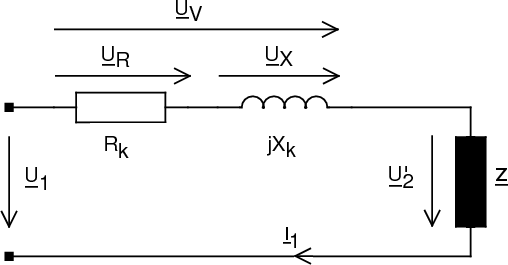
\includegraphics[width=5cm]{bilder/ErsatzschaltbildTrafoLast.png}
	            	\end{minipage}\\			
            \end{tabular}\\ \\

			\begin{tabular}{p{8cm}|p{10cm}}
	 			\textbf{Zeigerdiagramme} & \textbf{Kappsches Dreieck}\\
				\begin{minipage}{8cm}
	            	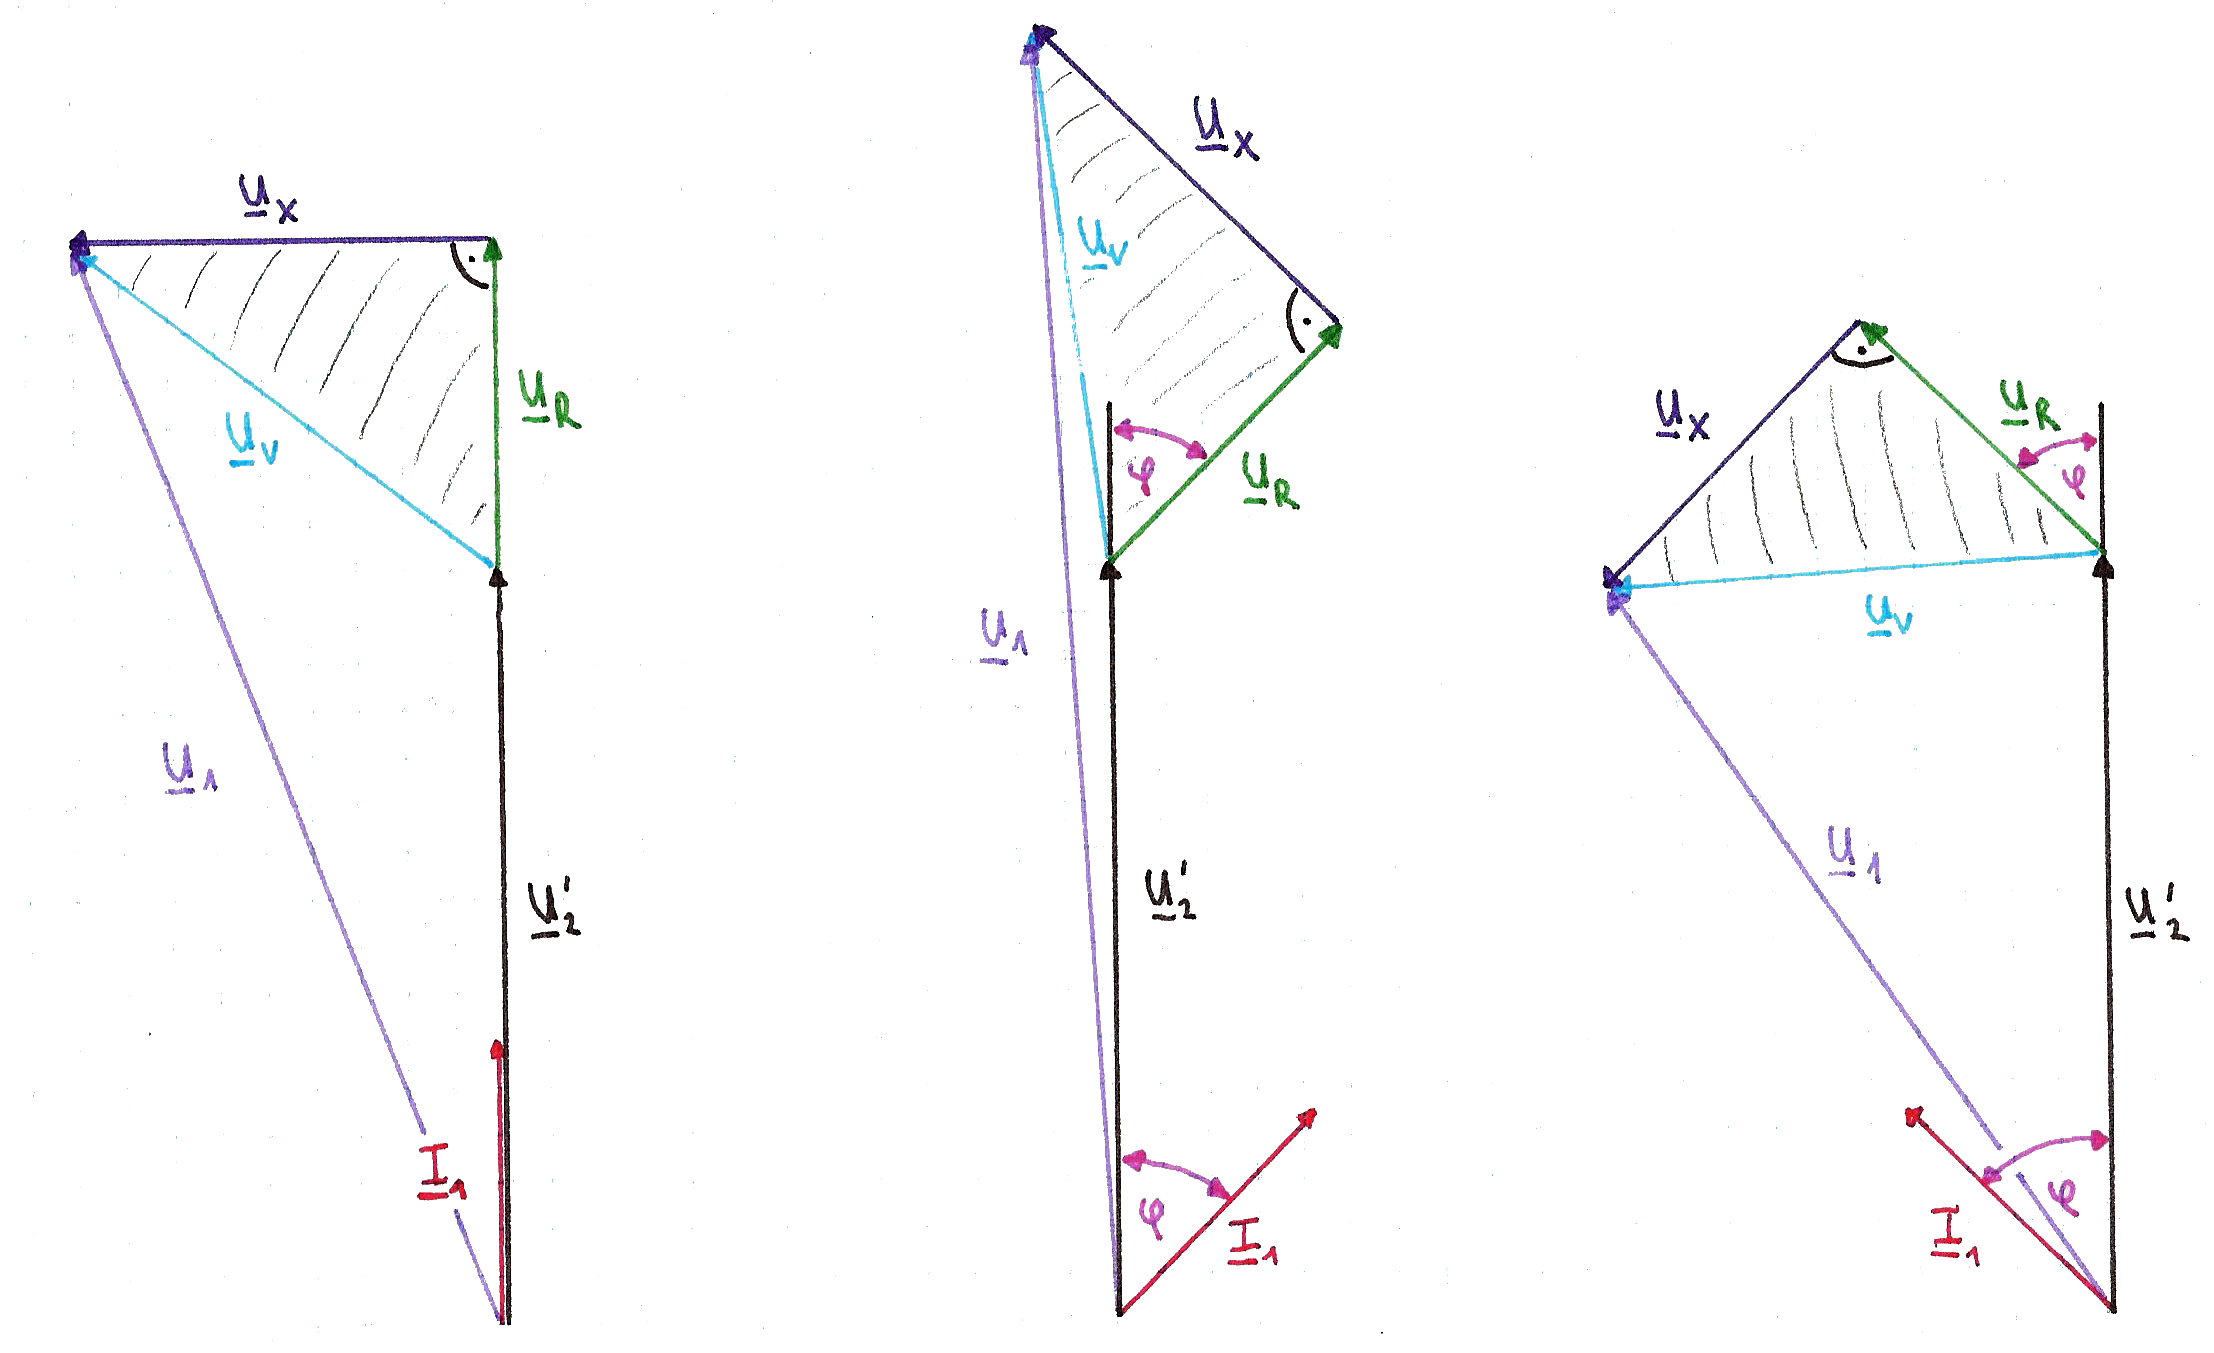
\includegraphics[width=8cm]{bilder/KappschesDreieck_1.png}
	            \end{minipage}  & \hspace{0.2cm}
				\begin{minipage}{10cm} 
		        	\begin{minipage}{2.5cm}
						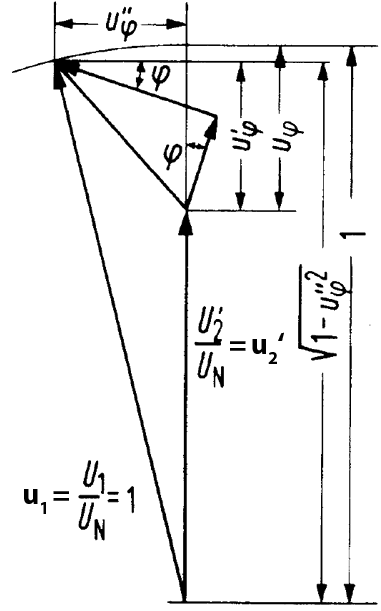
\includegraphics[width=3cm]{bilder/KappschesDreieck.png}
		            \end{minipage}
					\begin{minipage}{7.5cm}
		      			$$u_{\varphi} = u_{\varphi'} + 1 - \sqrt{1 - u_{\varphi''}^2}$$
		      			$$ u_\varphi \approx u_{\varphi'}\quad (\text{für }u_k
		      			=\frac{U_k}{U_{N}} \cdot 100\% < 4 \%)$$
		      			$$u_{\varphi'} = u_r \cdot \cos \varphi + u_x
		      			\cdot \sin \varphi$$ $$u_{\varphi''} = u_x \cdot \cos \varphi - u_r \cdot \sin \varphi$$
		      			$$ u_r = \frac{R_k I}{U_N} \qquad u_x = \frac{X_k I}{U_N} $$
		      			$$ U_2 = \frac{U_N}{"u} - \Delta U_2 = \frac{U_1}{"u} - \frac{1}{"u}
		      			U_N u_\varphi $$\\
		      		\end{minipage}         
                \end{minipage}\\
				\begin{minipage}{8cm}
 					\begin{tabular}[c]{p{2.66cm}p{2.66cm}p{2.66cm}}
                     	$\quad \varphi = 0$ & $\quad\varphi > 0$ & $\quad\varphi
                     	< 0$\\ rein ohmsche & induktive & kapazitive\\
                     	Last & Last & Last\\
                     	&&\\
                     	&&\\
                     	&&\\
                     	&&\\
                     \end{tabular}               
                \end{minipage}& \hspace{0.2cm}
				\begin{minipage}{10cm}
		      		Beim kappschen Dreieck wird mit ``genormten'' Gr\"ossen (klein $u$) gerechnet: 
		      		$u = \frac{U_{Strang}}{U_{N, Strang}} = \frac{U_X}{U_1} \qquad
		      		\boldsymbol{U_N = U_1} $\\ \\ Das Kappsche Dreieck dreht sich um die
		      		Spitze der Prim\"arspannung. Bei konstantem Strom und variablem $cos(\varphi)$ beschreibt ${u}_2'$
		      		einen
		      		Kreis um die Prim\"arspannung.\\ Bei \textbf{kapazitiver Last steigt}
		      		die Sekund\"arspannung über den Leerlaufwert an. \\                  
                \end{minipage}     
            \end{tabular}

		
		\subsubsection{Wirkungsgrad des Trafos}
			\begin{tabular}{p{5cm}p{7cm}p{7cm}}
            	Wirkungsgrad &
            		$\eta = 1-\dfrac{P_{V0} + P_{VK} \cdot
            		(\frac{P_B}{P_N})^2}{P_B} $ &
            	\begin{minipage}{7cm}
                	$P_B$ = Betriebsnennleistung\\
                	$P_{N}$ = Nennleistung\\
                	$P_{V0}$ = Leerlaufverlustleistung\\
                	$P_{VK}$ = Kurzschlussverlustleistung                	
                \end{minipage}\\ \\
            	 &
            		$\eta = 1 - \dfrac{a + (\frac{P_B}{P_N})^2}{P_B} P_{VK}$ &
            	\begin{minipage}{7cm}
 					$a = \dfrac{P_{V0}}{P_{VK}}$                	
                \end{minipage}\\ \\            		
            	 &
            		$\eta = 1 - \frac{P_{V0}+P_{VK}}{P_B} $ 
            		& (bei Wirkleistungsvollast) \\ \\
            	Maximaler Wirkungsgrad
            	& $S_{\eta-max} = \sqrt{a} \cdot S_N$ $P_{\eta-max} = \sqrt{a}
            	\cdot P_N$
            	& (Kupferverluste = Eisenverluste)
            \end{tabular}	

\newpage
	\subsection{Transformatoren Kühlmittel}
		\begin{center}
	    	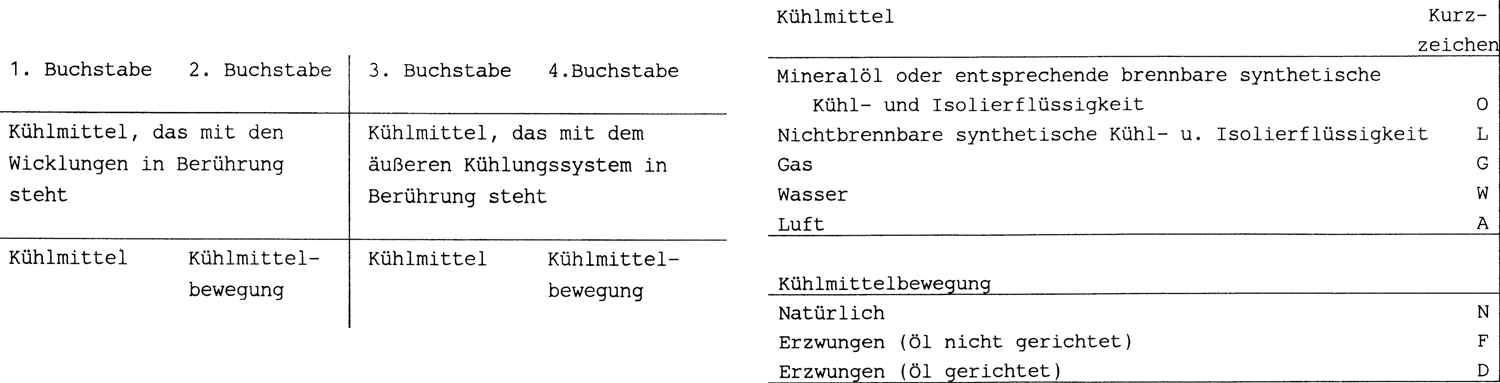
\includegraphics[width=19cm]{bilder/Kuehlmittel.png}
	    \end{center} 

	\subsection{Drehstrom-Leistungstransformatoren} 
	Angegebene Leistung bezieht sich immer auf alle drei Wicklungen. $\Rightarrow P_{Wicklung} =
	\frac{P_N}{3}$ \\
	Angegebene Spannungen und Str\"ome gelten immer für Aussenleiter. Somit muss immer entweder - je
 nachdem ob Dreieck- oder Sternschaltung vorliegt -	Strom oder Spannung mit Faktor
 $\frac{1}{\sqrt{3}}$ multipliziert werden.
 	\subsubsection{Bauformen}
	 $$\text{Kennzeichnung} = [a][b][c][d] = \begin{cases}
                  [a] = \text{Oberspannungswicklung, Grossbuchstabe (Y,D,III,Z)
                  }\\
                  [b] = \text{Unterspannungswicklung, Kleinbuchstabe (y,d,iii,z) } \\
                  [c] \cdot 30^\circ = \text{Phasenverschiebung zwischen Unter- und Oberspannung }
                  \\ [d] = 0 \text{, falls Neutralleiter herausgeführt (optional)}
                  \end{cases}$$
		\begin{center}
	    	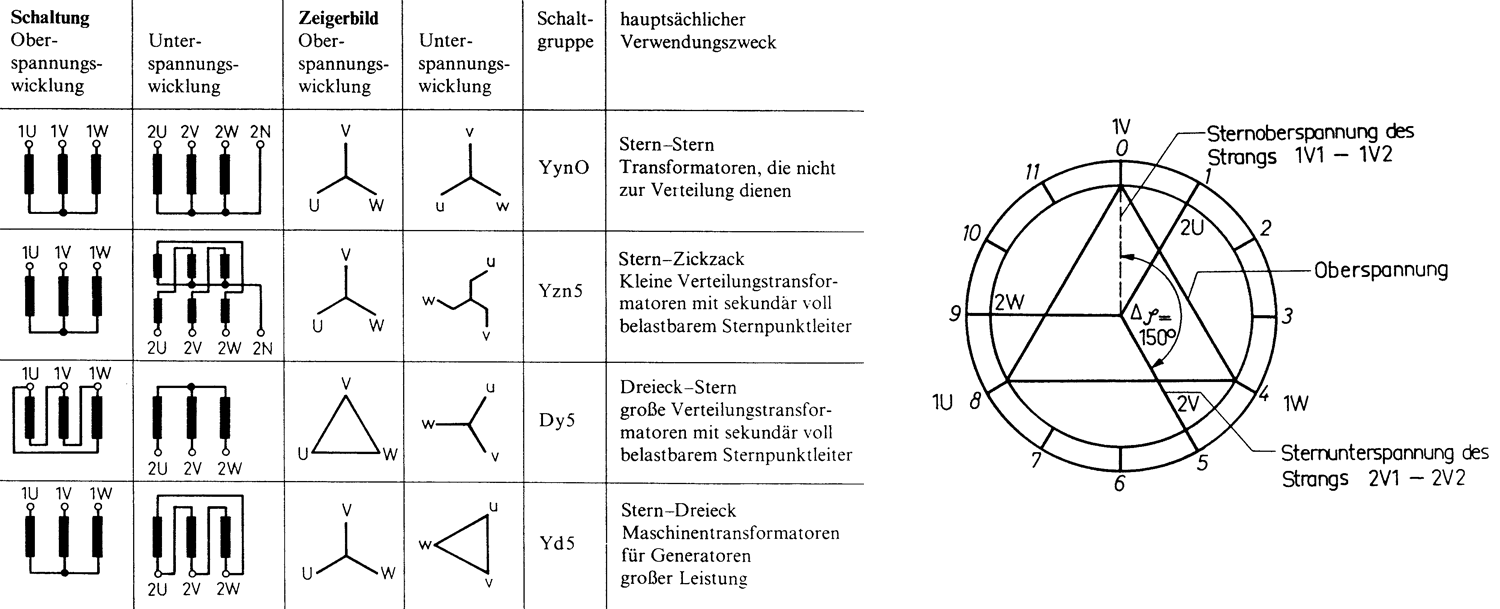
\includegraphics[height=6cm]{bilder/Drehstromtrafo.png}
	    \end{center} 

\newpage
\section{Dreiphasenwechselstrom (Drehstrom)}
	%\subsection{Entstehung des Drehstrom-Systems}
		\begin{tabular}{p{8.5cm}p{9cm}}
        	\begin{minipage}{8cm}
            	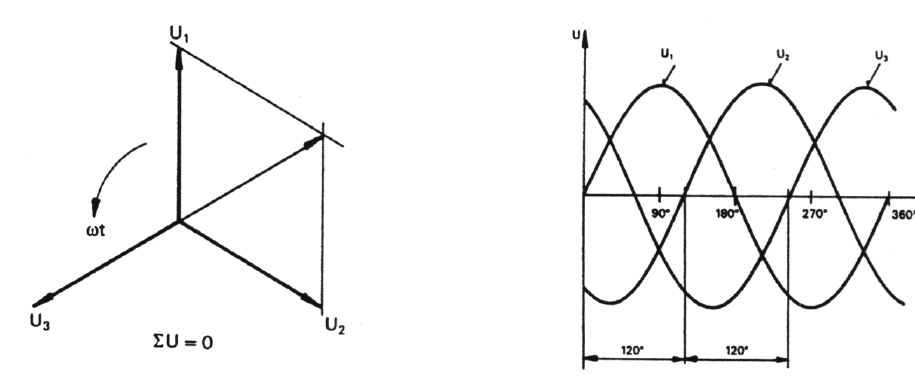
\includegraphics[width=7.5cm]{../WS_DST/bilder/Drehstrom.png}
            \end{minipage} &    
			\begin{minipage}{10cm}
            	Zeiger drehen mit $\omega t$ im Gegenuhrzeigersinn ($\omega > 0$). \\
            	$\underline{U}_2$ ist gegenüber $\underline{U}_1$ 
				$120^{\circ}$ nacheilend, $\underline{U}_3$ gegenüber $\underline{U}_1$ $240^{\circ}$.  \\ \\
				Somit gilt (bei symmetrischer Belastung): \\
				$\underline{U}_2 = \underline{U}_1 \cdot e^{j (-120^{\circ})}; \underline{U}_3
				= \underline{U}_1 \cdot e^{j (-240^{\circ})} = \underline{U}_1 \cdot e^{j
				(120^{\circ})}$
            \end{minipage}
        \end{tabular}
		
% 		\subsubsection{Verketten der Spannungen oder Str\"ome}
% 			\begin{tabular}{p{5cm}p{6cm}p{7cm}}
%             	\textbf{Maschensatz} &
%             		\fbox{$\underline{U}_1 + \underline{U}_2 + \underline{U}_3 = 0$} \\
%             	\textbf{Knotenpunktsatz} &
%             		\fbox{$\underline{I}_1 + \underline{I}_2 + \underline{I}_3 = 0$} \\
%             \end{tabular}

		\subsubsection{Stern- (Y) / Dreieckschaltung ($\Delta$)}
            	\renewcommand{\arraystretch}{1.5}
			\begin{tabular}{| p{4.5cm} | l | l |}
				\hline
	 				& Sternschaltung (Y)		& Dreieckschaltung ($\Delta$)\\
	 			\hline
	 			\vspace{0.2cm}
	 				%\textbf{Zeigerdiagramm} & & \\ 
	 				&
	 					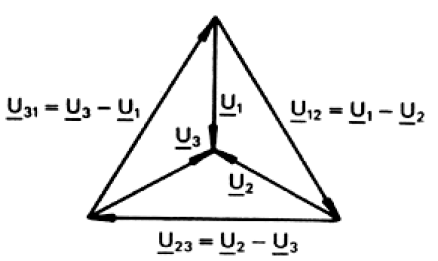
\includegraphics[width=5cm]{../WS_DST/bilder/Sternspannung.png} &
	 					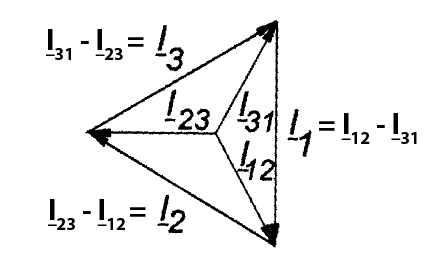
\includegraphics[width=5cm]{../WS_DST/bilder/Dreieckstrom.png} \\
	 				
		 			Verkettete Spannung &
		 				$U = U_{Str} \cdot \sqrt{3}$ \hspace{0.2cm} $\underline{U} = \underline{U}_{Str} \cdot \sqrt{3} \cdot e^{j 30^\circ}$ &
		 				$U = U_{Str}$ \hspace{0.2cm} $\underline{U} = \underline{U}_{Str}$ \\
		 			Aussenleiterstr\"ome &
		 				$I = I_{Str}$ \hspace{0.2cm} $\underline{I} = \underline{I}_{Str}$ &
		 				$I = I_{Str} \cdot \sqrt{3} $ \hspace{0.2cm} $\underline{I} =
		 				\underline{I}_{Str} \cdot \sqrt{3} \cdot e^{-j 30^\circ} $ \\ Gesamt-Scheinleistung &
		 				$S = 3 \cdot S_{Str} =\sqrt{3} \cdot U \cdot I $ \hspace{0.2cm} in $[VA]$
		 				& $S = 3 \cdot S_{Str} = \sqrt{3} \cdot U \cdot I$ \hspace{0.2cm} in $[VA]$ \\ Scheinleistung pro Strang &
		 				\multicolumn{2}{l|}{\hspace{3cm} $S_{Str} = U_{Str} \cdot I_{Str}$ \hspace{0.2cm} in $[VA]$} \\
		 			Wirkleistung &
		 				\multicolumn{2}{l|}{\hspace{3cm} $P = S \cdot \cos\varphi = \sqrt{3} \cdot U \cdot I \cdot \cos\varphi$ \hspace{0.2cm} in $[W]$} \\
		 			Blindleistung &
		 				\multicolumn{2}{l|}{\hspace{3cm} $Q = S \cdot \sin\varphi = \sqrt{3} \cdot U \cdot I \cdot \sin\varphi$ \hspace{0.2cm} in $[var]$} \\
% 		 			Wirkarbeit &
% 		 				\multicolumn{2}{l|}{\hspace{3cm} $W = P \cdot t = \sqrt{3} \cdot U \cdot I \cdot cos\varphi \cdot t$ \hspace{0.2cm} in $[Ws, kWh]$} \\
% 		 				&\multicolumn{2}{c|}{}\\
% 		 			Blindarbeit &
% 		 				\multicolumn{2}{l|}{\hspace{3cm} $W_b = Q \cdot t = \sqrt{3} \cdot U \cdot I \cdot sin\varphi \cdot t$ \hspace{0.2cm} in $[varh, kvarh]$} \\
	 			\hline
			\end{tabular}
        \renewcommand{\arraystretch}{1}
		
		%\subsubsection{Bestimmung des Y-Punktes mittels Leitwert-Operatoren im Vierleiter-Drehstromnetz}
        \subsubsection{Ausfall des Neutralleiters: Bestimmung des Y-Punktes mittels Leitwert-Operatoren}
            \begin{tabular}{p{5cm}p{13cm}}
            	\begin{minipage}{8cm}
                	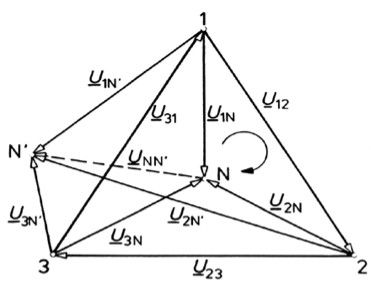
\includegraphics[width=5cm]{../WS_DST/bilder/ZeigerdarstellungVerschobenerSternpunkt.png}
                \end{minipage} &
				\begin{minipage}{13cm}
                	$\underline{U}_{12} = \underline{U}_{1N'} - \underline{U}_{2N'}$ \hspace{0.3cm}
                	$\underline{U}_{1N'} = \underline{U}_{1N} + \underline{U}_{NN'}$ \hspace{0.3cm}
                	$\underline{I}_1 = \underline{Y}_1 \cdot \underline{U}_{1N'} = \underline{Y}_1 \cdot (\underline{U}_{1N} + \underline{U}_{NN'})$ \\
                	$\underline{U}_{23} = \underline{U}_{2N'} - \underline{U}_{3N'}$ \hspace{0.3cm}
                	$\underline{U}_{2N'} = \underline{U}_{2N} + \underline{U}_{NN'}$ \hspace{0.3cm}
                	$\underline{I}_2 = \underline{Y}_2 \cdot \underline{U}_{2N'} = \underline{Y}_2
                	\cdot (\underline{U}_{2N} + \underline{U}_{NN'})$ \\ $\underline{U}_{31} = \underline{U}_{3N'} - \underline{U}_{1N'}$ \hspace{0.3cm}
                	$\underline{U}_{3N'} = \underline{U}_{3N} + \underline{U}_{NN'}$ \hspace{0.3cm}
                	$\underline{I}_3 = \underline{Y}_3 \cdot \underline{U}_{3N'} = \underline{Y}_3
                	\cdot (\underline{U}_{3N} + \underline{U}_{NN'})$ \\ \\ 
                	$$\underline{U}_{NN'} = \boldsymbol{-} \frac{(\underline{Y}_1 \cdot
                	\underline{U}_{1N} + \underline{Y}_2 \cdot \underline{U}_{2N} + \underline{Y}_3 \cdot
                	\underline{U}_{3N})}{\underline{Y}_1 + \underline{Y}_2 +
                	\underline{Y}_3}$$
                \end{minipage}
			\end{tabular}

%		\subsubsection{Anwendung der Y- und $\Delta$- Schaltung}
	
	\subsection{Stern-Dreieck-Umwandlung}% \formelbuch{18}}
	%\begin{figure}
	  \begin{minipage}[lt]{7.5 cm}
	    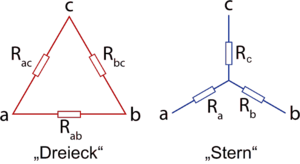
\includegraphics[width=6cm]{bilder/stern-dreieck.png} 
	  \end{minipage}
	  \begin{minipage}[rt]{9.35 cm} %BASTEL!!
      \renewcommand{\arraystretch}{2}
	  \begin{tabular}{ll}
	Umwandlung $\triangle \rightarrow Y$: 
		&$Z_{c} = \dfrac{Z_{ac} Z_{bc}}{Z_{ab}+Z_{bc}+Z_{ac}}$\\
	Umwandlung $Y \rightarrow \triangle$: 
		&$Y_{ac}=\dfrac{Y_{a} Y_{c}}{Y_{a}+Y_{b}+Y_{c}}$\\
	Bei gleichen Widerst\"anden:
	&$R_Y = \frac{R_\triangle}{3}$ \\
	Bei gleichen Kapazit\"aten:
	&$C_Y = C_\triangle \cdot 3 $ \\
	Bei gleichen Induktivit\"aten:
	&$L_Y = \frac{L_\triangle}{3}$
	  \end{tabular}
      \renewcommand{\arraystretch}{1}
	  \end{minipage}
	%\end{figure}
	
	\subsection{Defektleistung von symmetrischen Drehstromverbrauchern}
		\begin{tabular}{| p{7.5cm} | l | l |}
			\hline
 				& Normalleistung		& Defektleistung\\
 			\hline
	 			\textbf{Y-Schaltung bei Leiter- oder Strangausfall} ohne Neutralleiter &
	 				$P_{Norm} = 3 \cdot \frac{U^2_{Str}}{R} = \frac{U^2}{R}$ &
	 				$P_{Def} = \frac{1}{2} \frac{U^2}{R}$ \tiny{nur 50\% von $P_{Norm}$} \\
	 			&&\\
	 			\textbf{Y-Schaltung bei Leiter- oder Strangausfall} mit Neutralleiter &
	 				$P_{Norm} = 3 \cdot \frac{U^2_{Str}}{R} = \frac{U^2}{R}$ &
	 				$P_{Def} = 2 \cdot \frac{U^2_{Str}}{R} = \frac{2}{3} \frac{U^2}{R}$ \tiny{nur 66\% von
	 				$P_{Norm}$} \\ &&\\
	 			\textbf{$\Delta$-Schaltung bei Leiterausfall} &
	 				$P_{Norm} = 3 \cdot \frac{U^2}{R}$ &
	 				$P_{Def} = \frac{U^2}{R} + \frac{U^2}{2R} = \frac{3U^2}{2R}$ \tiny{nur 50\% von $P_{Norm}$} \\
	 			&&\\
	 			\textbf{$\Delta$-Schaltung bei Strangausfall} &
	 				$P_{Norm} = 3 \cdot \frac{U^2}{R}$ &
	 				$P_{Def} = 2 \cdot \frac{U^2}{R}$ \tiny{nur 66\% von $P_{Norm}$} \\
	 		\hline
		 \end{tabular} 
\section{Wissenswertes}
\begin{itemize}
	\itemsep0.5em
	\item Netzspannungsschwankung = $\pm 10 $
	\item Impedanzverhältnis $R_{Q}/X_{Q}=0.1$
	\item Netzspannung = verkettete Spannung
	\item Strangspannung = Spannung gegenüber 0
\end{itemize}
%TODO: Fehlerrechnung ->Aus Praktikum 1

\newpage
\section{Beispiele}
\subsection{Gleichrichter}
\begin{multicols}{2}
\subsubsection{Einweggleichrichter}
Ungesteuerter Einweggleichrichter M1U: \newline
Ventil/Diode und Trafo werden als verlustlos betrachtet.
\adjustbox{scale=1}{\begin{circuitikz}[european ]
	\draw 
	(0,0) node[transformer] (T) {}
	(T.base) node {$\frac{N_1}{N_2}$};
	\draw (T.A1) to[short, i_=$I_1$] +(-0.5,0) node[circ] {};
	\draw (T.A2) to[short] +(-0.5,0) node[circ] {};
	\draw (T.B1) to[short, i=$I_s$] ++(0.5,0) to[D] ++(1,0) to[short] ++(0.5,0) 
		to[short, i=$I_d$] ++(0,-0.5) to[R] ++(0,-1.2) |- (T.B2); 
		
	\draw[->, thick] (-1.6,-0.25) -- ++(0,-1.6) node[midway, left] {$U_1$};
	\draw[->, thick] (0.9,-0.25) -- ++(0,-1.6) node[midway, right] {$U_s$};
	\draw[->, thick] (2.6,-0.25) -- ++(0,-1.6) node[midway, left] {$U_d$};
	\draw (-0.5,-2.4) node  {$S_{1Tr}$};
	\draw (0.5,-2.4) node  {$S_{2Tr}$};
\end{circuitikz}}

\renewcommand{\arraystretch}{1.5}
\begin{tabular}{ll}
	Mittelwert $U_d$ 				& $ = \frac{\hat{U}_s}{\pi}$ \\
	Mittelwert $I_d$ 				& $ = \frac{U_d}{R}$ \\
\end{tabular}

\begin{tabular}{ll}
	Effektifvert $I_s$				& $ = \frac{\hat{U}_s}{2R}$ \\
	Wirkleistung Last $P_L$			& $ = I_s^2 \cdot R$ \\
	Leistungsaufnahme $S_{2Tr}$		& $ = U_s \cdot I_s$ \\
	Leistungsaufnahme $S_{1Tr}$		& $ = U_1 \cdot 1.21 \cdot I_d \frac{1}{"u}$ \\
	Primärstrom $I_1$				& $ \approx I_d \cdot \frac{1.21}{"u} $ \\
	Bauleistung $S_{Tr}$			& $ = \frac{S_{1Tr} + S_{2Tr}}{2}$ \\
	Stromgrundschwingung $I_{s1}$	& $ = \frac{P}{U_s \cdot \cos\varphi_1}$ ,($\varphi_1 = 0$) \\
	Spitzenstrom in Ventil $\hat{i}$& $ = \hat{i}_d = \frac{\sqrt{2} U_s}{R}$ \\
\end{tabular}
\end{multicols}

\begin{multicols}{2}
\subsubsection{Dimmer (Triac, W1C)}
Ventile verlustlos, Steuerwinkel = $90^\circ$ \newline
\adjustbox{scale=1}{\begin{circuitikz}[european]
	\draw (0,0) node [circ, name=in] {};
	\draw (0,-2) node[circ, name=out] {};
	\draw (in) -- +(1,0) node[circ, name=p1] {};
	\draw (p1) -- ++(0,0.5) to[D] ++(1.2,0) -- ++(0,-1) to[D] ++(-1.2,0) -- +(0,0.5) ;
	\draw (2.2,0) node[circ] {} to[short, i=$I_S$] ++(1.4,0) to[R=R] ++(0,-2) -- (out);
	\draw[->, thick] (0,-0.25) -- ++(0,-1.6) node[midway, left] {$U_N$};
	\draw[->, thick] (3,-0.25) -- ++(0,-1.6) node[midway, left] {$U_A$};
\end{circuitikz}}

\renewcommand{\arraystretch}{1.5}
 \begin{tabular}{ll}
 	Effektivspannung $U_A$		& $ = U_N \cdot \sqrt{\frac{1}{2}}$ \\
 	Effektivstrom $I_S$			& $ = \frac{U_A}{R}$ \\
 	Wirkleistung $P_R$			& $ = \frac{U_A^2}{R} $ \\
 	Leistungsaufname $S_N$		& $ = U_N \cdot I_S $ (Winkel: $45^\circ$) \\
 	Leistungsfaktor $\lambda$	& $ = \cos \varphi = 0.707 $\\
 	Blindleistung $Q$			& $ = \sqrt{S_N^2 -P_R^2}$\\
 \end{tabular}
 \end{multicols}
 
 \begin{multicols}{2} 
 \subsubsection{Brückengleichrichter B2U}
 Ventile/Dioden und Trafo verlustlos! \newline
 \adjustbox{scale=1}{\begin{circuitikz}[european]
	\ctikzset{voltage/distance from node=.7}% in \pgf@circ@Rlen units 
	\ctikzset{voltage/distance from line=.3}% pos. between 0 and 1 
	\ctikzset{voltage/bump b/.initial=1.5}% 
	\draw 
		(0,0) node[transformer] (T) {} 
		(T.A1) to[short, i_=$I_1$] ++(-0.5,0) node[circ] {}
		(T.A2) to[short] +(-0.5,0) node[circ] {};
	
	\draw (T.B1) 
		to[short, i=$I_s$] ++(0.8,0) node[circ, name=is] {} 
		to[D, v^>=$U_{V1}$] ++(0,2) to[short] ++(1,0) node[circ] {} 
		to [short] ++(3,0) 
		to[short, i=$I_d$] ++(0,-1.5) 
		to[R=R] ++(0,-2.5) |- ++(-3,-1.5) node[circ, name=b1] {} 
		to [short] ++(-1,0) 
		to[D, l=V3] ++(0,1.4) -- (is) ; 
	\draw (T.B2) to[short] ++(1.8,0) node[circ, name=b2] {} to[short] ++(0,2.1) to[D, l_=V2] ++(0,2);
	\draw (b1) to[D, l_=V4] (b2);
		
	\draw[->, thick] (-1.6,-0.25) -- ++(0,-1.6) node[midway, left] {$U_1$};
	\draw[->, thick] (1.4,-0.25) -- ++(0,-1.6) node[midway, left] {$U_s$};
	\draw[->, thick] (4.5,1.75) -- ++(0,-5) node[midway, left] {$U_d$};
\end{circuitikz}}
 
 \renewcommand{\arraystretch}{1.5}
 \begin{tabular}{ll}
 	Mittelwert $U_d$						& $ = 2 \cdot \frac{\hat{U}_s}{\pi}$ \\
 	Mittelwert $I_d$						& $ = \frac{U_d}{R}$ \\
 	Effektivwert $I_{d,eff}$				& $ = \frac{U_{d,eff}}{R} = \frac{\sqrt{2} U_s}{\sqrt{2} R}$ \\
 	Effektivwert Ventilstrom $I_{V,eff}$	& $ = \frac{\hat{U}_s}{2 R} = \frac{U_s}{\sqrt{2} R}$ \\
 	Leistung $P_R$							& $ = R \cdot I_{d,eff}$ \\
 	Leistungsaufnahme $S_{TR}$				& $ = P_R $ Wenn alles ideal!
 \end{tabular} 
 \end{multicols}


\newpage
\section{Übungen}
\subsection{Übung 1: Mittelwerte}\label{ueb1}
\begin{center}
\includegraphics[width = 0.5\textwidth]{bilder/a1}
\end{center}

\begin{minipage}[t]{0.49\textwidth}
\begin{align*}
	i_n(t)&= \frac{i_{n+1}-i_n}{t_{n+1}-t_n}\cdot (t-t_n)+i_n&&t=0\textrm{ ergibt Offset}\\
	i_1(t) &= 0&&=0\\
	i_2(t)&= \frac{2}{0.0025}\cdot (t-0.0025) &&= 800\cdot t-2\\
	i_3(t)&= 2&&=2\\
	i_4(t)&= \frac{-3}{0.0025}\cdot (t-0.0075) +2&&=-1200\cdot t+11\\
	i_5(t)&=-1&&=-1\\
	i_6(t)&=\frac{1.5}{0.0025}\cdot (t-0.0125)-1&&=600\cdot t -8.5\\
	i_7(t)&=0.5&&=0.5\\
	i_8(t)&=\frac{-0.5}{0.0005}\cdot (t-0.0175)+0.5&&=-1000\cdot t+18
\end{align*}
\end{minipage}\begin{minipage}[t]{0.49\textwidth}
\begin{align*}
	u_n(t)&= \frac{u_{n+1}-u_n}{t_{n+1}-t_n}\cdot (t-t_n)+u_n\\
	u_1(t)&= 0\\
	u_2(t)&= \frac{2}{0.0025}\cdot(t-0.0025)+8&&=800\cdot t+6\\
	u_3(t)&= 2&&=2\\
	u_4(t)&=\frac{-3}{0.0025}\cdot (t-0.0075)-10&&=-1200\cdot t-1\\
	u_5(t)&=-1&&=-1\\
	u_6(t)&=\frac{-1.49}{0.0025}\cdot (t-0.0125) +5&&=596\cdot t-2,45\\
	u_7(t)&=0.5&&=0.5\\
	u_8(t)&=\frac{-0.5}{0.0005}\cdot(t-0.00175)-9.5&&=-1000\cdot t+8
\end{align*}
\end{minipage}

\textbf{linearer Mittelwert} $I_{AV}\;,\;U_{AV}$
\[
I_{AV}= \frac{1}{T}\left(\int_{t_1}^{t_2} i_1(t) dt + \int_{t_2}^{t_3} i_2(t) dt +\ldots\right) \quad U_{AV} =\frac{1}{T} \left(\int_{t_1}^{t_2} u_1(t) dt + \int_{t_2}^{t_3} u_2(t) dt +\ldots\right)
\]

\textbf{Effektivwert} $I_{eff}\;,\;U_{eff}$
\[
I_{eff}= \sqrt{\frac{1}{T}\left(\int_{t_1}^{t_2} i_1(t)^2 dt + \int_{t_2}^{t_3} i_2(t)^2 dt +\ldots\right)} \quad U_{eff} =\sqrt{\frac{1}{T} \left(\int_{t_1}^{t_2} u_1(t)^2 dt + \int_{t_2}^{t_3} u_2(t)^2 dt +\ldots\right)}
\]

\textbf{Berechnung der Momentanleistung} $p(t)$\\
Es ist, gleich wie bei dem Strom und der Spannung eine Fallunterscheidung für die einzelnen Zeitbereiche zu machen.
\[
 p(t) = u(t)\cdot i(t) \left\lbrace 
 \begin{array}{rrr}
 p_1(t)&=0&0\leq t\leq 0.0025\\
 P_2(t)&=\dfrac{2}{0.0025}\cdot(t-0.0025)+8\cdot\dfrac{2}{0.0025}\cdot(t-0-0025)&0.0025\leq t\leq 0.005\\
 p_3(t) &= 2\cdot 2&0.005\leq t \leq 0.0075\\
 p_4(t)&=\dfrac{-3}{0.0025}\cdot (t-0.0075)-10 \cdot \dfrac{-3}{0.0025}\cdot (t-0.0075)+2&0.0075\leq t\leq 0.010\\
 \vdots&\vdots&\vdots
 \end{array}
 \right.
\]

\textbf{Berechnung der Wirkleistung}
\begin{align*}
P&=\frac{1}{T}\int_0^T(u(t)\cdot i(t)) dt = \frac{1}{T}\int_0^T p(t)dt\\
P&=\frac{1}{T}\left(\int_{0}^{0.0025}p_1(t)dt + \int_{0.0025}^{0.005}p_2(t)dt + \int_{0-005}^{0.0075}p_3(t)dt + \int_{0.0075}^{0.010}p_4(t)dt +\ldots\right)
\end{align*}

\textbf{Berechnung der effektiven Welligkeit des Stromes}
\[
	\textrm{Welligkeit } = \dfrac{\textrm{Effektivwert des Wechselanteils}}{\textrm{Gleichrichtwert}}	= \frac{\i_{\sim eff}}{i_{av}} \quad \textrm{wobei: } i_{\sim}(t) = i(t) - i_{av}
\]


\subsection{Übung 2: Generator}

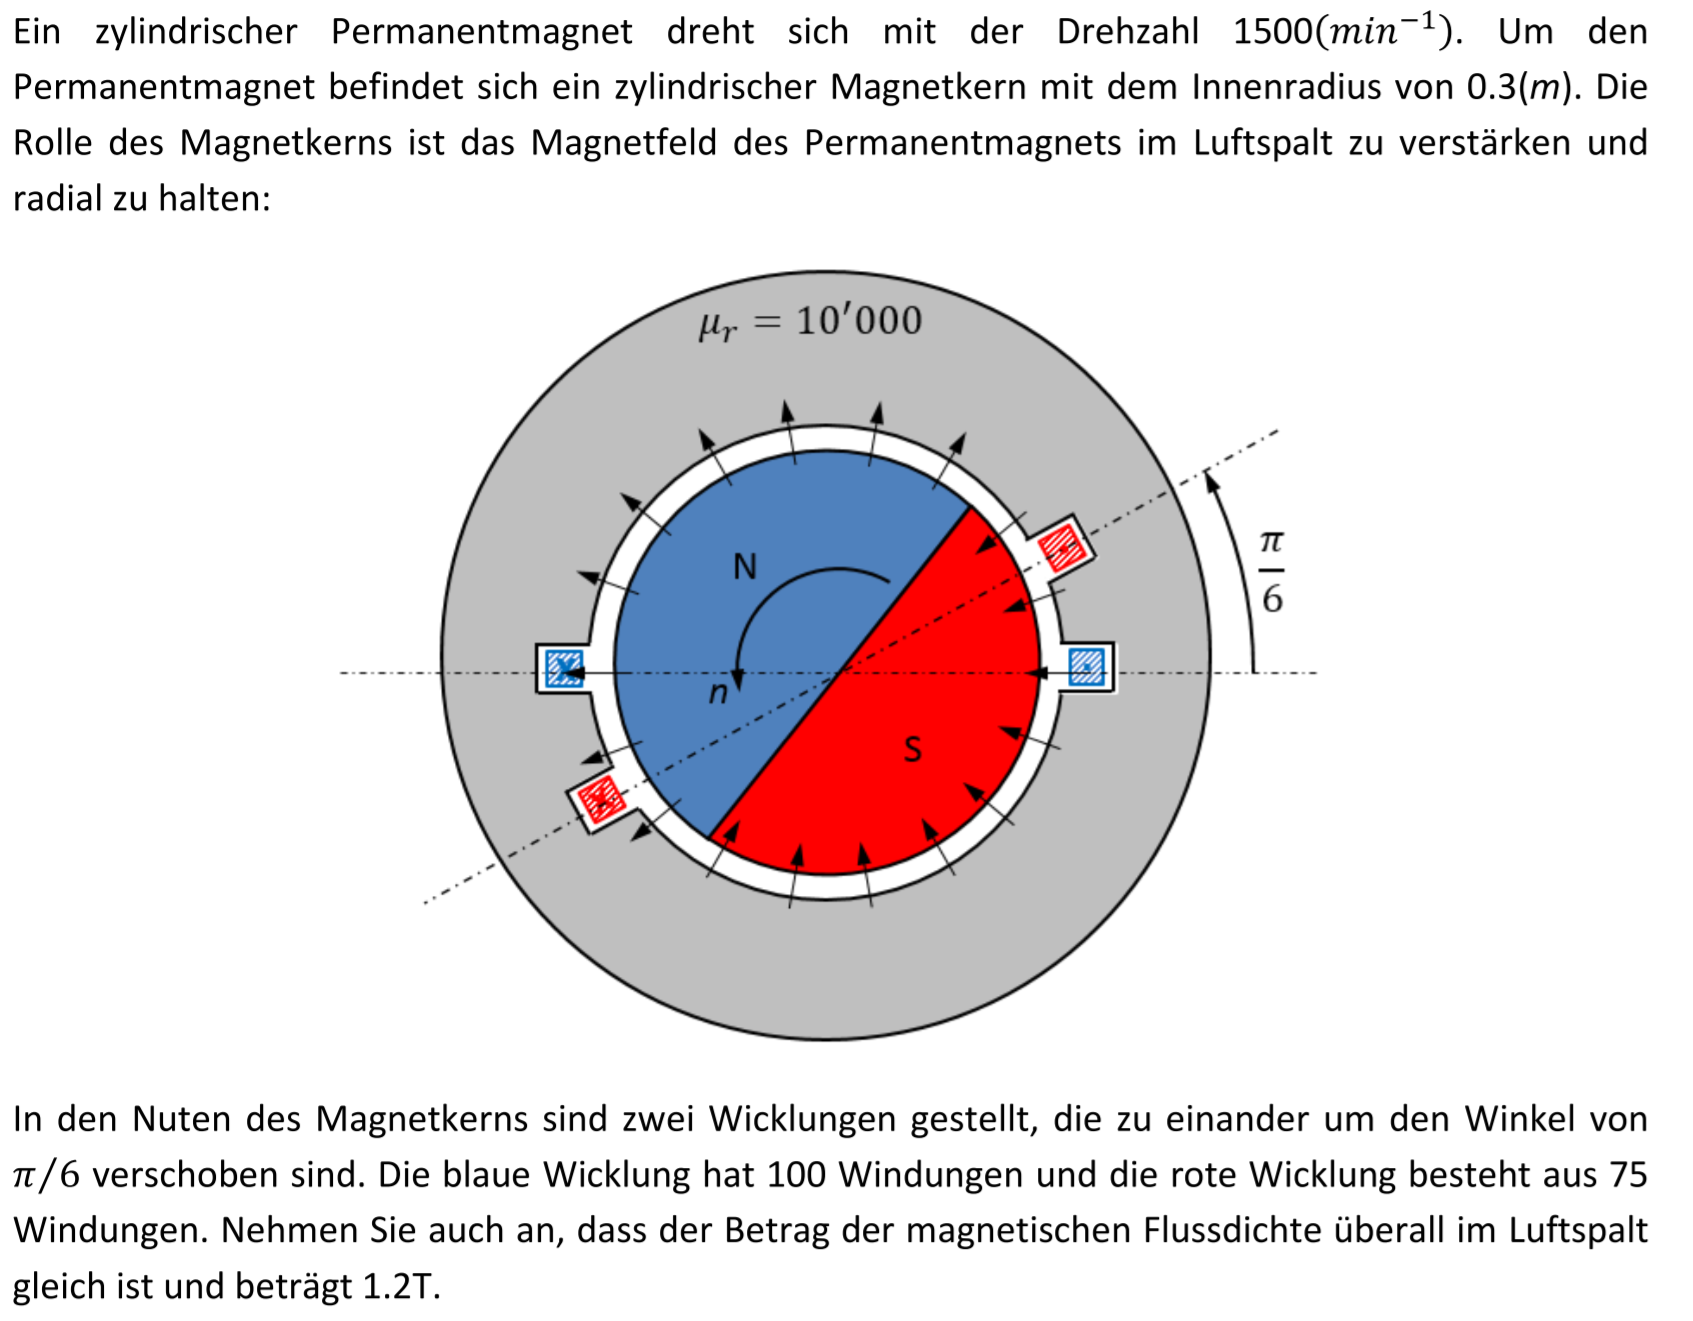
\includegraphics[width = 0.8\textwidth]{bilder/a21.png}

Um den magnetischen Fluss darstellen zu können muss man sich vorstellen dass der Fluss um die Spule fliessen muss, was bei einer konstanten Flussdichte direkt von der Fläche abhängig ist.
\begin{align*}
	\Phi_{blau}(\alpha) &= B \cdot r\cdot  l \cdot (\pi - \alpha) -  B\cdot r\cdot l\cdot \alpha = B \cdot r\cdot  l \cdot (\pi - 2\cdot \alpha) &(0\leq \alpha \leq \pi)\\
	\Phi_{blau}(\alpha) &=  -B \cdot r\cdot  l \cdot (3\pi - 2\cdot \alpha) &(\pi\leq \alpha \leq 2\pi)\\
	\Phi_{rot}(\alpha) &= B \cdot r\cdot  l \cdot (\pi - 2\cdot \alpha+\frac{\pi}{3}) &(\frac{\pi}{6}\leq \alpha \leq \frac{7\pi}{6})\\
	\Phi_{rot}(\alpha) &= -B \cdot r\cdot  l \cdot (3\pi - 2\cdot \alpha+\frac{\pi}{3}) &(\frac{7\pi}{6}\leq \alpha \leq \frac{13\pi}{6})
\end{align*}
	
Die induzierte Spannung ist nun $u(t) = L\dfrac{di(t)}{dt} = -N\dfrac{d\Phi}{dt}$

\begin{align*}
	u_{blau}(t) &= -N\frac{d\Phi}{dt} = -N\cdot B \cdot r  \cdot l\cdot \left(\pi - \frac{2 \pi\cdot n \cdot t}{60} \right) \frac{1}{dt}\qquad = N\cdot B \cdot r\cdot l \cdot \pi \frac{n}{15} &(0\leq \alpha \leq \pi)\\
	u_{blau}(t) &= -N\frac{d\Phi}{dt} = N\cdot B \cdot r  \cdot l\cdot \left(\pi - \frac{2 \pi\cdot n \cdot t}{60} \right) \frac{1}{dt}\qquad = -N\cdot B \cdot r\cdot l \cdot \pi \frac{n}{15} &(\pi\leq \alpha \leq 2\pi)\\
\end{align*}
Die Spannung für die rote Spule wird gleich berechnet, einfach erneut um $\frac{\pi}{6}$ Phasenverschoben.


\newpage
\subsection{Lineare elektrische Netzwerke}
\begin{minipage}{0.35\textwidth}
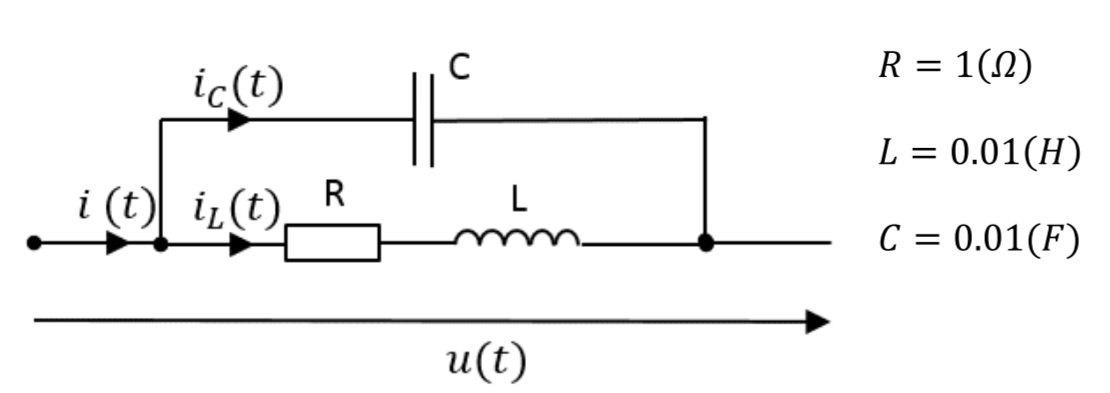
\includegraphics[width=0.9\textwidth]{bilder/a31.png}
\end{minipage}
\begin{minipage}{0.64\textwidth}
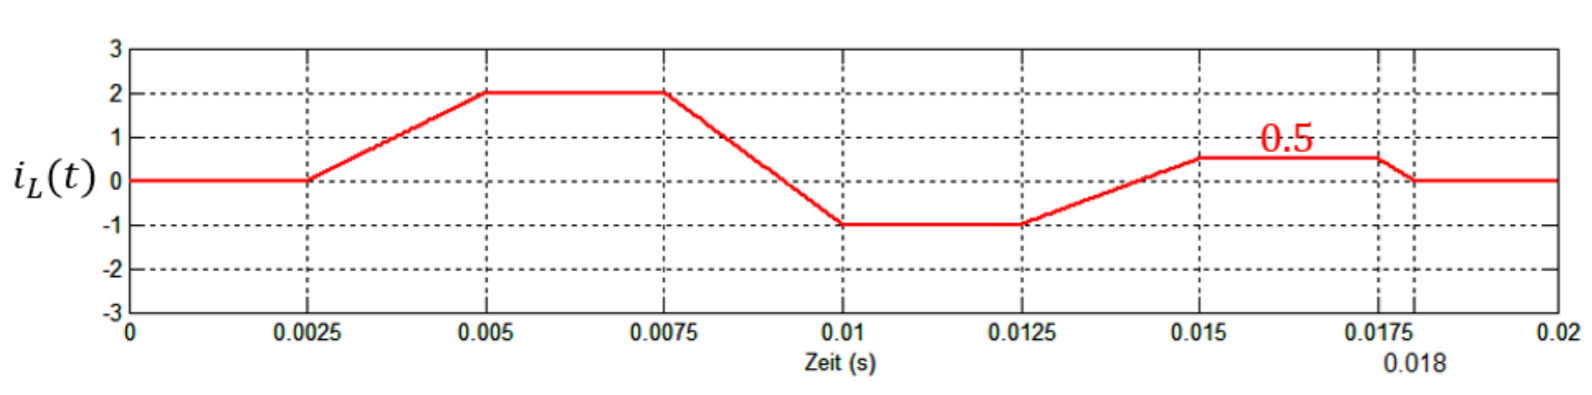
\includegraphics[width=0.9\textwidth]{bilder/a32.png}
\end{minipage}

Die gegebenen Ströme sind die Ströme über dem Spulenpfad. Die Funktionen sind gemäss Aufgaben 1 auf Seite \pageref{ueb1}

Gesucht sind \begin{itemize}
\itemsep0em
\item $u(t)$
\item $i_c(t)$
\item $i(t)$
\item Eintrag ins Diagramm
\end{itemize}

\begin{minipage}{0.49\textwidth}
\begin{align*}
u(t)&=R\cdot i(t)+L\cdot \frac{di}{dt}\\
u_1(t)&=0&&=0\\
u_2(t)&=800\cdot t -2+0.01\cdot 800&&=800\cdot t+6\\
u_3(t)&=2&&=2\\
u_4(t)&=-1200\cdot t+11 +0.01\cdot (-1200)&&=-1200\cdot t -1\\
\vdots&=\vdots
\end{align*}
\end{minipage}
\begin{minipage}{0.49\textwidth}
\begin{align*}
i_c&= C\cdot \frac{du}{dt}\\
i_1(t)&=0&&=0\\
i_2(t)&=0.01\cdot 800&&=8\\
i_3(t)&=0&&=0\\
i_4(t)&=0.01\cdot (-1200)&&=-12\\
\vdots&=\vdots
\end{align*}
\end{minipage}
\vspace{5mm}
$i(t)$ ist nun nur die Summe der Serieschaltung und des Kondensators: $i(t) = i_c(t) + i_L(t)$

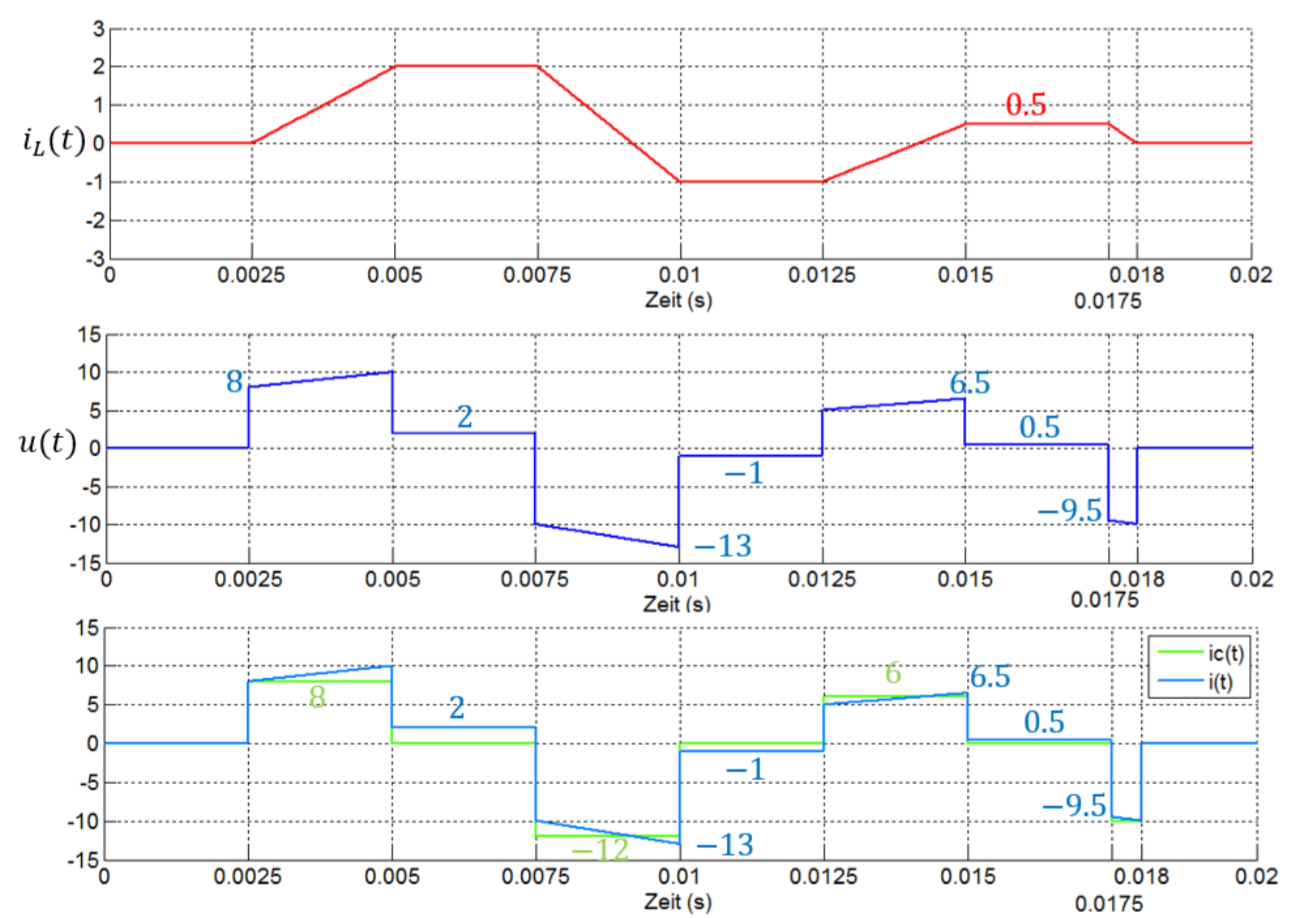
\includegraphics[width=0.95\textwidth]{bilder/a33.png}

\newpage
\subsection{Symbolische Methode}
\includegraphics[width=0.6\textwidth]{bilder/a41.png}
\begin{enumerate}
\item Berechnen sie die komplexen Ströme $i_1 , i_C, i_M$ der Schaltung.\\
Es wird das Maschenstromverfahren angewendet. Die linke Fenstermasche ist $J_1$, die rechte Fenstermasche ist $J_2$. Umlaufsinn ist jeweils der Uhrzeigersinn. Es wird jeweils mit den Effektivwerten gerechnet
\[
	\left[
	\begin{array}{lll}
	j\omega (L_N+L_L) + \frac{1}{j\omega C_K}+ (R_N+R_L)&-\frac{1}{j\omega C}&U_N\\
	-\frac{1}{j\omega C} & j\omega L_M + R_M+\frac{1}{j\omega C}&0
\end{array}		
	\right] \;\textrm{ mit }\omega = 2\pi 50Hz \; = \left[
	\begin{array}{lll} 
		1&0&29.504-j\cdot 13,792\\
		0&1&29.008-j\cdot 20.56 	
	\end{array}\right]
\]
\[
	\begin{array}{lll}
		i_1&= J_1 &= 29.504-j\cdot 13,792\\
		i_C&= J_1-J_M &= 0.498+j\cdot 6.768\\
		i_M&=J_2&= 29.008-j\cdot 20.56
	\end{array}
\]
\item Berechnen sie die Schein-, Wirk-, und Blindleistung der Schaltung

\begin{minipage}{0.5\textwidth}
\begin{align*}
	S&=U_{eff}\cdot I_{eff}^* = I_1\cdot U_N &= (6785,9+j\cdot 
3172,12)VA\\
	P&=\texttt{real(s)} &= 6785.9W\\
	Q&=\texttt{imag(S)} &= 3172,1 VAr 
\end{align*}
\end{minipage}

\item Berechnen sie den Leistungsfaktor $\cos (\varphi)$ der Schaltung

\begin{minipage}{0.5\textwidth}
\begin{align*}
	\varphi &= \texttt{angle(S)} &= -25,05^\circ\\
	cos(\varphi) &= \texttt{cos(angle(S))} &= 0.905
\end{align*}
\end{minipage}

\item Stellen sie das Zeigerdiagramm der Schaltung dar

\begin{minipage}{0.5\textwidth}
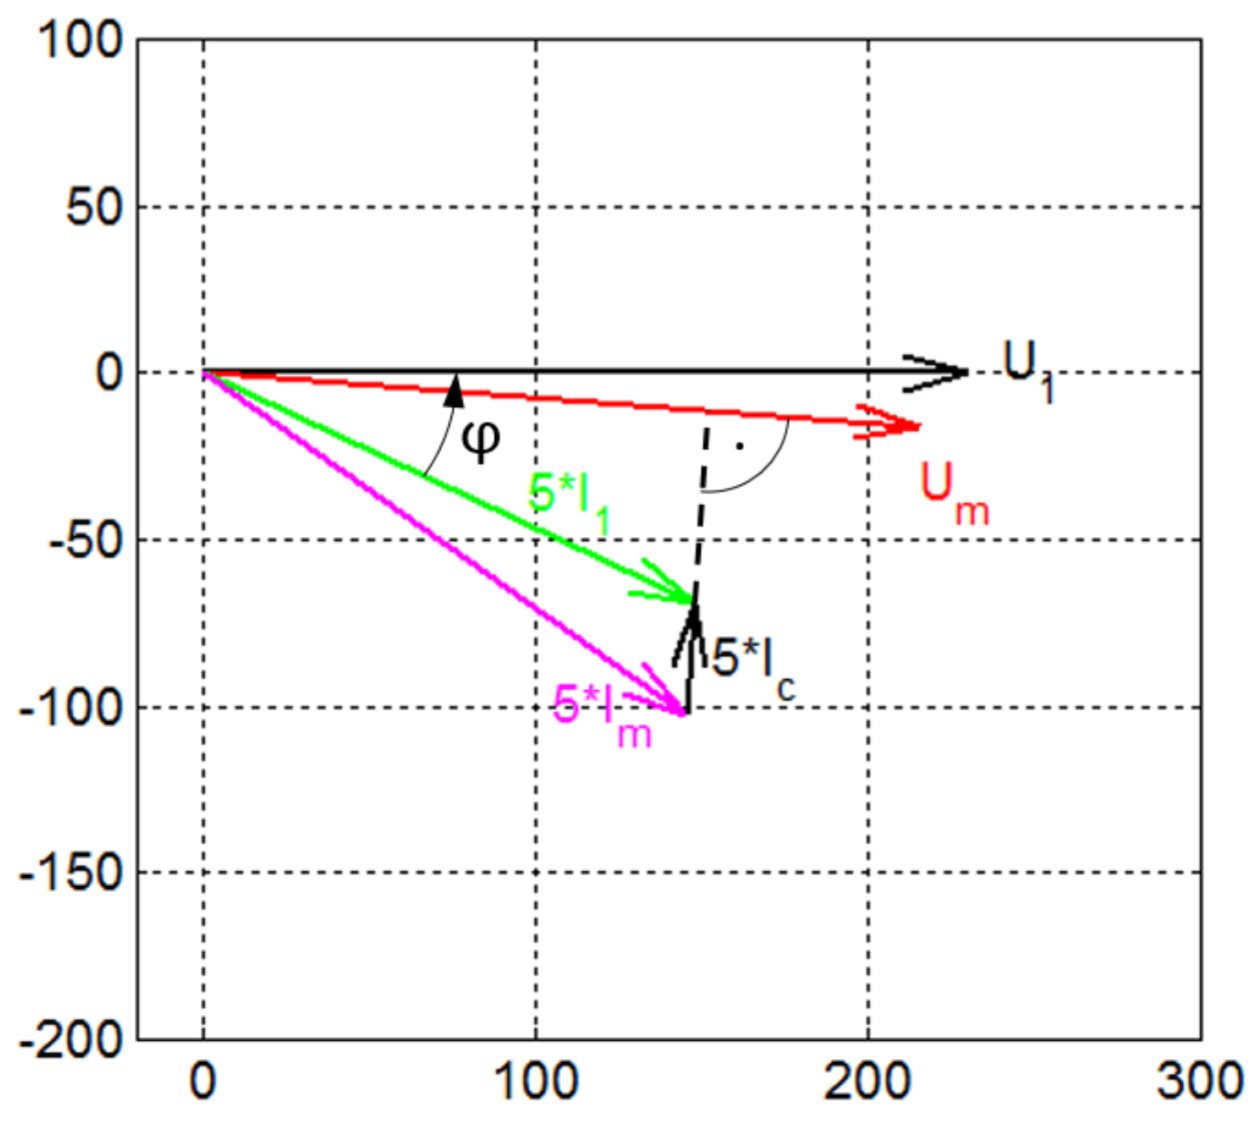
\includegraphics[width=0.9\textwidth]{bilder/a42.png}
\end{minipage}
\begin{minipage}{0.45\textwidth}
Die Ströme aus Aufgabe 1 sind massstabsgetreu einzuzeichnen mit Betrag und Winkel
\end{minipage}

\item Berechnen sie den Kondensator für einen $\cos(\varphi) = 0$\\
Damit der $\cos(\varphi)$ = 1 ist muss der Imaginäranteil der Schaltung = 0 sein. Nicht mit \texttt{pwider(\ldots,\ldots)} arbeiten!

\[
	Z = \left( R_n+R_L + j\omega (L_N+L_L) +\frac{\frac{1}{j\omega C}\cdot (j\omega L_M+R_M)}{\frac{1}{j\omega C}+ (j\omega L_M+R_M)}\right)=0 \quad \texttt{solve(\ldots,C)}
\]

\end{enumerate}
\begin{minipage}[]{0.7\textwidth}
    \begin{circuitikz}
   	  \draw (0,0)
   	  node[rground]{}
   	  to[I, i_=$i(t)$](0,4) node[ocirc]{} node[above]{$E_A$} 
   	  to[R=$R_L$](4,4)
   	  to[L=$L_L$](6,4)
   	  to[short](8,4)
   	  to[R=$R_M$](8,2)
   	  to[L=$L_M$](8,0)
   	  node[rground]{}
   	  ;
      \draw (6,4) node[ocirc]{} node[above]{$E_B$} 
      to[C=$C_K$](6,0)
      node[rground]{}
      ;
    \end{circuitikz}
    
    \end{minipage}
\begin{minipage}[]{0.29\textwidth}
Wobei:\\
- $R_L = 0.2\Omega$\\
- $L_L = 0.1\mu H$\\
- $C_K = 8.3\mu F$\\
- $R_M = 2\Omega$\\
- $L_M = 10mH$\\
- $i(t) = \sqrt{2}\cdot 60A\cdot \sin(2\pi\cdot 50\cdot t)$\\
$+\sqrt{2}\cdot 7A\cdot \sin(2\pi\cdot 250\cdot t)$\\
$+\sqrt{2}\cdot 5A\cdot \sin(2\pi\cdot 550\cdot t)$
\end{minipage}
    \vspace{5mm}
    
    Knotenpotentialmethode:
\[
	\left[\begin{array}{cc}
		\dfrac{1}{R_L+j\omega L_L}&-\dfrac{1}{R_L+j\omega L_L}\\
		-\dfrac{1}{R_L+j\omega L_L}&\dfrac{1}{R_L+j\omega L_L} +\dfrac{1}{R_M+j\omega L_M}+j\omega C_K
	\end{array}\right]
	\cdot \left[\begin{array}{c}
	E_A\\E_B
	\end{array}\right]
	= \left[\begin{array}{c}
	I_{50,250,550}\\0
	\end{array}\right] \vert \omega = 2\pi f
\]
\[
	\left[\begin{array}{cc}
		\dfrac{1}{0.2\Omega+j\omega \cdot 0.1\mu H}&-\dfrac{1}{0.2\Omega+j\omega \cdot 0.1\mu H}\\
		-\dfrac{1}{0.2\Omega+j\omega \cdot 0.1\mu H}&\dfrac{1}{0.2\Omega+j\omega \cdot 0.1\mu H} +\dfrac{1}{2\Omega+j\omega \cdot 10mH}+j\omega 8.3\mu F
	\end{array}\right]
	\cdot \left[\begin{array}{c}
	E_A\\E_B
	\end{array}\right]
	= \left[\begin{array}{c}
	I_{50,250,550}\\0
	\end{array}\right] \vert \omega = 2\pi 50,250,550
\]
\[
	\underbrace{\left[\begin{array}{cc}
	E_A(50Hz)=&328.115V\angle 54.725^\circ\\
	E_B(50Hz)=&318.618V\angle 57.217^\circ
	\end{array}\right]}_{\textrm{ungefährlich da} < \sqrt{2}\cdot 230V}
	\underbrace{\left[\begin{array}{cc}
	E_A(250Hz)=&197.346V\angle 80.298^\circ\\
	E_B(250Hz)=&197.021V\angle 80.866^\circ
	\end{array}\right]}_{\textrm{ungefährlich da} < \sqrt{2}\cdot 230V}
	\underbrace{\left[\begin{array}{cc}
	E_A(550Hz)=&4218.93V\angle 5.403^\circ\\
	E_B(550Hz)=&4217.52V\angle 5.405^\circ
	\end{array}\right]}_{\textrm{Gefährlich da} > \sqrt{2}\cdot 230V}
\]
Optional mit Impedanz und Strömen lösen
\begin{align*}
Z(\omega) &= R_L +j\omega L_L +\frac{1}{j\omega C_M +\frac{1}{R_M+j\omega L_M}} \qquad\vert \omega = 2\cdot \pi \cdot 50, 2\cdot \pi \cdot 250,2\cdot \pi \cdot 550\\
U_M(\omega)&= Z(\omega) \cdot I(\omega)
\end{align*}
\hrule

\begin{minipage}[]{0.7\textwidth}
    \begin{circuitikz}
   	  \draw 
   	  (4.5, 2.5) node[transformer] (T) {}
   	  (0,3)node[ocirc]{} 
   	  to [short,i=$I_1$](1,3)--(3,3) -- (T.A1)
   	  (4, 1.425) node[left] {$N_1$}
      (5, 1.425) node[right] {$N_2$}
      (1.5,3) to [C=$C$](1.5,0)
      (0,3) to [open, v=$U_1$](0,0)
      (T.A2) -- (3,0) -- (0,0)node[ocirc]{}
      (T.B1) -- (6,3) -- (9,3) to [R=$R_L$](9,0) -- (6,0)--(T.B2)
      (7.5,3) to [L=$L_L$](7.5,0)
      (7,3) to [open,v=$U_L$] (7,0)
      ; 
    \end{circuitikz}
\end{minipage}
\begin{minipage}[]{0.29\textwidth}
	\begin{itemize}
	\itemsep0em
	\item $L_L = 0.05H$
	\item $R_L = 15\Omega$
	\item $u(t) = 230V\angle 0^\circ$
	\item $f= 50Hz$
	\item ü $ = \frac{N_1}{N_2} = 8$
	\item $\varphi_k = 0.839$
	\end{itemize}
\end{minipage}


\begin{circuitikz}[american]
\begin{scope}[]
\draw [->] (-1,0) -- (3,0) node[anchor=west] {$P/W$};
\draw [->] (0,-0.5) -- (0,3) node[anchor=west] {$Q/VAr$} ;
\draw [->] (0,0) -- (2.755,0)node[anchor=north] {$P$};
\draw [->] (2.755,0) -- (2.755,2.631)node[anchor=west] {$Q$};
\draw [->] (0,0) -- (2.755,2.631)node[anchor=south east] {$S$};
\draw [->] (2.755,2.631) -- (2.755,1.780)node[anchor=west] {$Q_C$};
\draw [thick,->] (0,0) -- (2.755,1.780)node[anchor=south east] {$S_K$};
%\draw (-1,0) node[anchor=north] {-2} (1,0) node[anchor=south] {2}
%(0,1) node[anchor=west] {4} (0,-1) node[anchor=east] {-4}
%(2,0) node[anchor=north west] {4}
%(-1.5,0) node[anchor=south east] {-3};
%\draw [thick] (-2,-1) -- (-1,1) -- (1,-1) -- (2,0) -- (2.5,.5);
%\draw [dotted] (-1,1) -- (-1,0) (1,-1) -- (1,0)
%(-1,1) -- (0,1) (1,-1) -- (0,-1);
\end{scope}
\end{circuitikz}


\begin{align*}
\underline{Z}_2' &=\underline{Z}_2\cdot \left(\frac{N_1}{N_2}\right)^2  =\frac{1}{\frac{1}{R} +\frac{1}{j\omega L}}\cdot 8^2 =  \frac{1}{\frac{1}{15} +\frac{1}{j 2\pi 50Hz\cdot 0.05H}}\cdot 64 &&= 694.288\Omega\angle 43.679^\circ\\
\underline{I}_1 &= \frac{\underline{U}}{\underline{Z}'_2} = \frac{230V\angle 0^\circ}{694.288\Omega\angle 43.679^\circ} &&=  0.3312A\angle-43.679^\circ\\
\underline{S} &= \underline{U}\cdot \underline{I}_1^*=(230V\angle 0^\circ) \cdot (0.3312A\angle 43.679^\circ)&&= 76.193VA\angle 43.679^\circ\\
P &= \texttt{Real}(S) = \texttt{Real}(76.193VA\angle 43.679^\circ)&&=55.104W\\
Q &= \texttt{Imag}(S) = \texttt{Imag}(76.193VA\angle 43.679^\circ)&&=52.621VAr\\
C &= -\frac{P\cdot (\tan(\arccos(\cos(\varphi_K))-\tan(\varphi))}{\omega \cdot \underline{U}^2} = -\frac{55.104W\cdot (\tan(\arccos(0.839))-\tan(43.679^\circ))}{\omega\cdot (230V\angle 0^\circ)^2}&&=1.016\mu F
\end{align*}

\newpage

\begin{align*}
\underline{U}_{1N} &= 230.94V \angle 0^\circ\\
\underline{U}_{2N} &= 230.94V \angle -120^\circ\\
\underline{U}_{3N} &= 230.94V \angle -240^\circ\\
\underline{Z}_1&= 7\Omega + j\cdot 2\cdot \pi \cdot 50 Hz\cdot 0.3H\\
\underline{Z}_2&= 3\Omega\\
\underline{Z}_3&= 7\Omega\\
\underline{U}_{NN}'&= -\frac{\left( \underline{Y}_1\cdot \underline{U}_{1N} +\underline{Y}_2\cdot \underline{U}_{2N} +\underline{Y}_3 \cdot \underline{U}_{3N} \right)}{\underline{Y}_1+\underline{Y}_2+\underline{Y}_3}\\
 &= -\frac{\frac{1}{(7\Omega + j 2 \pi 50 \cdot 0.3H)}\cdot (230.94V \angle 0^\circ) +\frac{1}{3\Omega}\cdot (230.94V \angle -120^\circ)+\frac{1}{7\Omega} \cdot (230.94V \angle -240^\circ) }{\frac{1}{7\Omega + j\cdot 2\cdot \pi \cdot 50 Hz\cdot 0.3H}+\frac{1}{3\Omega}+ \frac{1}{7\Omega}}\\
&= 142.293V\angle 37.75^\circ\\
U_{1N}' &=U_{1N} + U_{NN}' = (230.94V\angle0^\circ) + (142.293V\angle 37.75^\circ) = (353.412V\angle 14.271^\circ)\\
U_{2N}' &=U_{2N} + U_{NN}' = (230.94V\angle -120^\circ) + (142.293V\angle 37.75^\circ) = (112.093V\angle -91.275^\circ)\\
U_{1N}' &=U_{1N} + U_{NN}' = (230.94V\angle -240^\circ) + (142.293V\angle 37.75^\circ) = (286.317V\angle 90.499^\circ)\\
\end{align*}

\hrule
\vspace{5mm}


\begin{minipage}[]{0.8\textwidth}
\begin{circuitikz}[american inductors]
\draw (0,2) to[sV=$\underline{U}_1$] (0,0)
to[short,i=$I_1$] (2,0)node[ocirc]{}
(2,0) -- (6,0)node[circ]{}
-- (8,0)node[circ]{}
--(14,0)node[ocirc]{}
(0,2) --(2,2)node[ocirc]{}
 	to[R=$R_1$](4,2)
 	to[L=$L_{1\sigma}$](6,2)node[circ]{}
 	to[R=$R_{FE}$](6,0)
(8,2) to[L=$L_{M}$](8,0)
(6,2) --(8,2)node[circ]{} --(8,4)
(8,2)to[L=$L_{2\sigma}'$](10,2)
	to[R=$R_2'$] (12,2)
	to[short,i=$I_2$](13,2)node[ocirc]{}
(8,4)to[L=$L_{3\sigma}'$](10,4)
	to[R=$R_3'$] (12,4)
	to[short,i=$I_3$](14,4)node[ocirc]{}
(13,2)to[open,v^=$\underline{U}_2'$](13,0)
(14,4)to[open,v^=$\underline{U}_3'$](14,0) 
;
\end{circuitikz}


\end{minipage}
\begin{minipage}{0.19\textwidth}
Nennbetrieb:
\begin{itemize}
\itemsep0em
\item $U_1 = 230V$
\item $f= 50$Hz
\item $U_2 = $ 24V
\item $U_3 = $ 12V
\item $P_1 = P_2+P_3+P_{FE} +P_{CU}$
\item $P_2 = 1.7kW$
\item $P_3 = 1.3kW$
\end{itemize}
\end{minipage}

\vspace{5mm}
\begin{minipage}{0.49\textwidth}
Leerlauftest:
\begin{itemize}
\itemsep0em
\item $S_0 = P_{FE} + j\cdot Q_\mu$
\item  $\qquad = 75W +j\cdot 95 VAr$
\end{itemize}
\end{minipage}
\begin{minipage}{0.49\textwidth}
Kurzchluss an $U_2, U_3$
\begin{itemize}
\item $S_K = P_{cu}+j\cdot Q_\sigma$
\item $ \qquad= 110W+ j\cdot 120 VAr$
\end{itemize}
\end{minipage}

\begin{align*}
R_{FE} &= \frac{U_1^2}{P_{FE}} = \frac{(230V)^2}{75W} = 705.333\Omega\\
L_M &= \frac{U_1^2}{Q_\mu\cdot \omega} = \frac{(230V)^2}{95VAr\cdot 2\pi\cdot 50Hz} = 1.77H\\
I_{2K} &=  \frac{P_2}{U_{2N}} = \frac{1700W}{24V} = 70.833A\\
I_{1K} &= \frac{P_3}{U_{3n}} = \frac{1300W}{12V} = 108.333A\\
Z_K^*&= \frac{U_0^2}{S_K} = \frac{(230V)^2}{(110W+ j\cdot 120 VAr)} = (219.355 -j\cdot 239.547)\Omega\\
R_1 &= R'_2\vert \vert R'_3\quad\Rightarrow = \frac{\texttt{Real}(Z_K)}{2} = 109.79\Omega\\
X_{\sigma 1}&= X'_{\sigma 2} \vert \vert X'_{\sigma 3}\quad \Rightarrow = \frac{\texttt{Imag}(Z_K)}{2} = 119.774\Omega\\
\end{align*}

\newpage





\subsection{Trafo Vol 1.0}
Gegeben sind folgende Daten:
\begin{itemize}
\itemsep0em
\item Primärspannung $U_1 = 32kV$, Sekundärspannung $U_2 = 400V$
\item Scheinleistung des Trafos $S = 1MVA$
\item Fläche des Eisenkerns $A_{FE} = 0.05m^2$
\item Maximale Flussdichte des Eisens $\hat{B} = 1.8T$
\item Streureaktanzen $X_{\sigma 1} = 30\Omega$, $X_{\sigma 2} = 7m\Omega$ 
\end{itemize}
\begin{enumerate}
\item Berechnen sie die Anzahl Windungen der Primär und Sekundärwicklung
\begin{align*}
U_{10} = \frac{2\pi}{\sqrt{2}} N_1\cdot f\cdot \hat{B} \cdot A_{FE} \Rightarrow N_1&= \frac{U_{10}\cdot \sqrt{2}}{2\cdot \pi \cdot f\cdot \hat{B} \cdot A_{FE}} &&= \frac{32'000V\cdot \sqrt{2}}{2\pi\cdot 50\cdot 1.8T\cdot 0.05m^2}=1600.56 \textrm{ Windungen}\approx	1601\\
N_2 &= \frac{U_{20}\cdot \sqrt{2}}{2\cdot \pi\cdot f\cdot \hat{B}\cdot A_{FE}}&&=\frac{400V\cdot \sqrt{2}}{2\pi\cdot 50\cdot 1.8T\cdot 0.05m^2}=20 \textrm{ Windungen}
\end{align*}
	
\item Berechnen sie den Primär und Sekundärstrom
\begin{align*}
I_1&=\frac{P}{U_1} &&=\frac{1\cdot10^6VA}{32'000V} = 31.25A\\
I_2&=\frac{P}{U_2} &&=\frac{1\cdot10^6VA}{400V} = 2500A
\end{align*}

\item Berechnen sie die Wicklungsverluste über der Primär und Sekundärwicklung wenn der Primärwiderstand $R_{10} = 20\Omega$ und der Sekundärwiderstand $R_{20} = 8m\Omega$ beträgt
\[
	P_W = P_{W1} + P_{W2} = I_1^2\cdot R_1+I_2^2\cdot R_2 = (31.25A)^2\cdot 20\Omega +(2500A)^2\cdot 0.008\Omega = 19.531kW+50kW = 69.531kW
\]
Wichtig: Über den Strom rechen da die Spannung auch den magnetischen Teil enthält der nicht in Wärme umgesetzt wird.

\item Berechnen sie den Wirkungsgrad des Transformators im Nennbetrieb wenn die Leerlaufleistung $P_L = 30kW+j\cdot 40kVAr$
\[
	\eta = \frac{P_{ab}}{P_{zu}} = \frac{S-P_W-P_L}{S} = \frac{1000kW-69.531kW-30.000kW}{1000kW} \cdot 100\%= 90.04\% 
\]

\newpage
\item Zeichen sie das Vollständige Zeigerdiagramm des Trafos bei Nennlast.

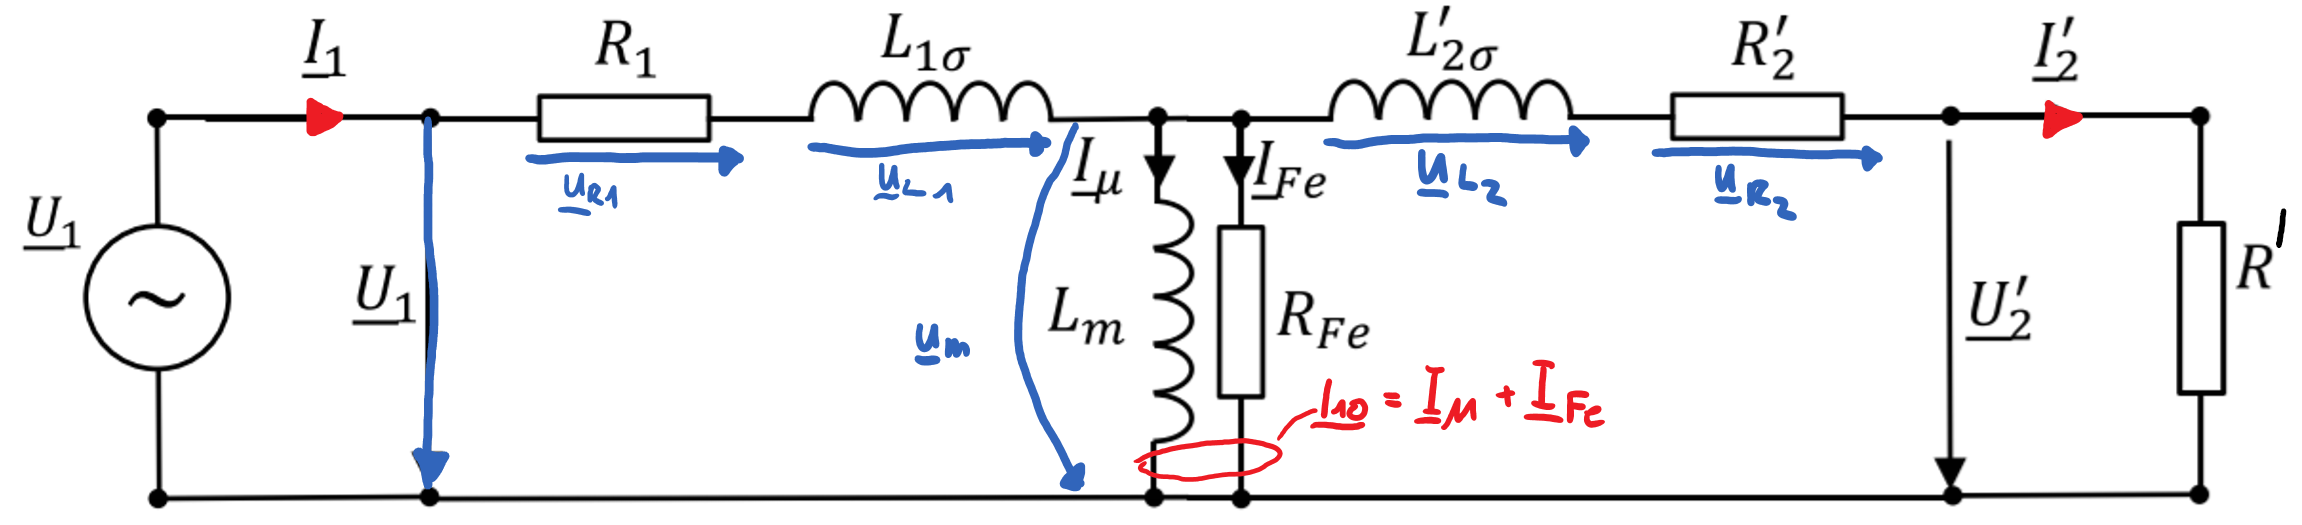
\includegraphics[width=0.99\textwidth]{bilder/a52.png}

\begin{minipage}{0.49\textwidth}
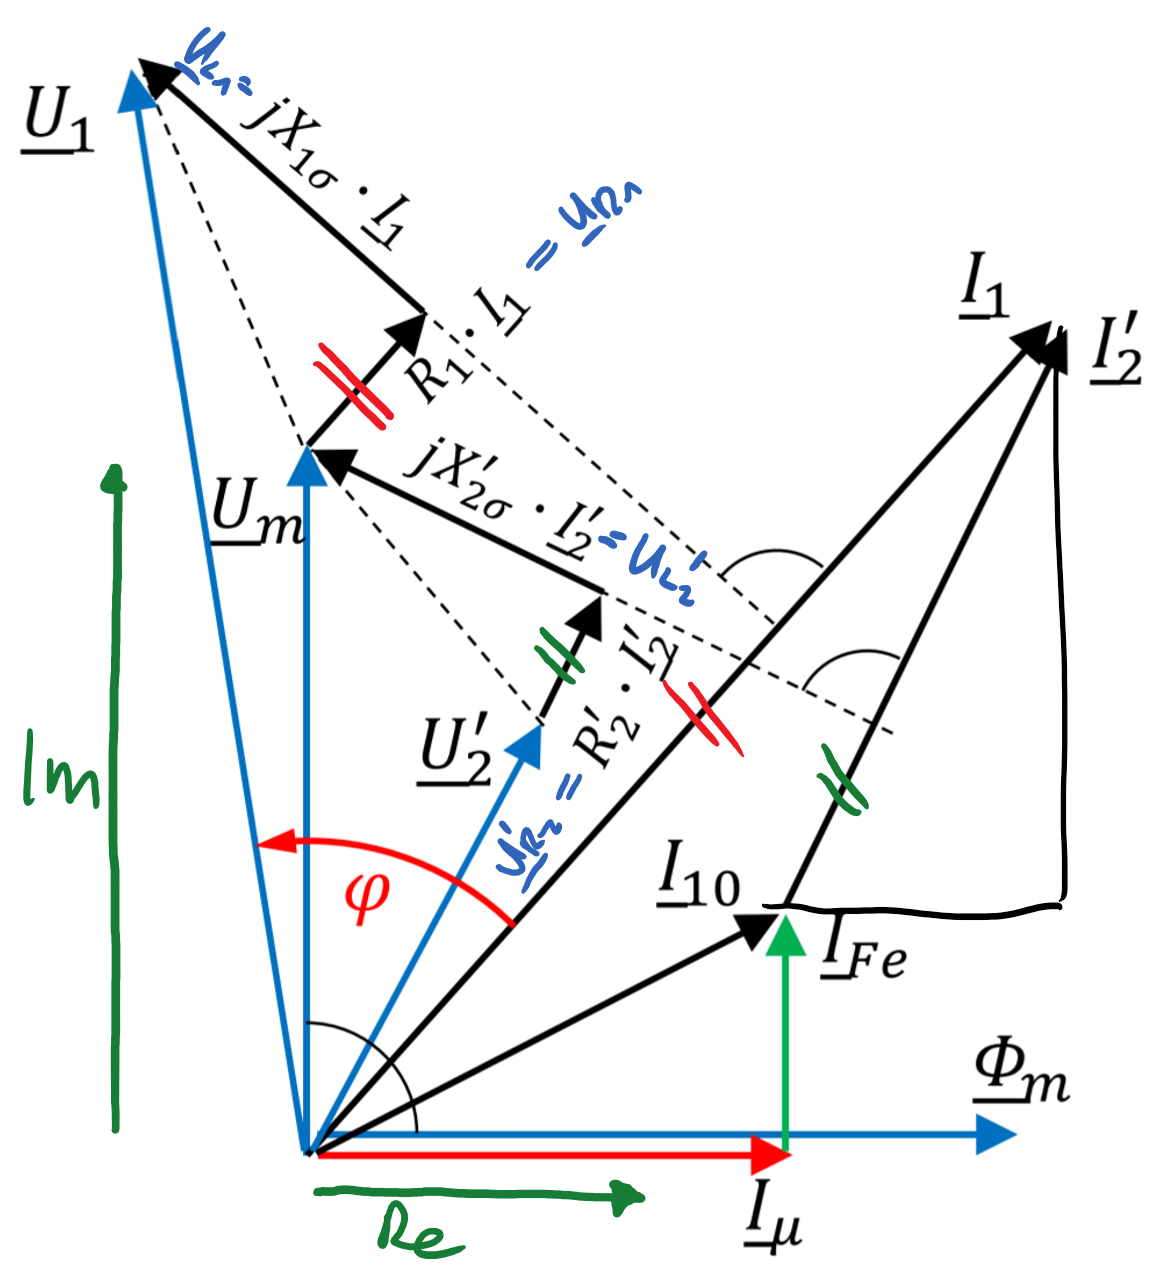
\includegraphics[width=0.7\textwidth]{bilder/a53.png}
\end{minipage}
\begin{minipage}{0.49\textwidth}
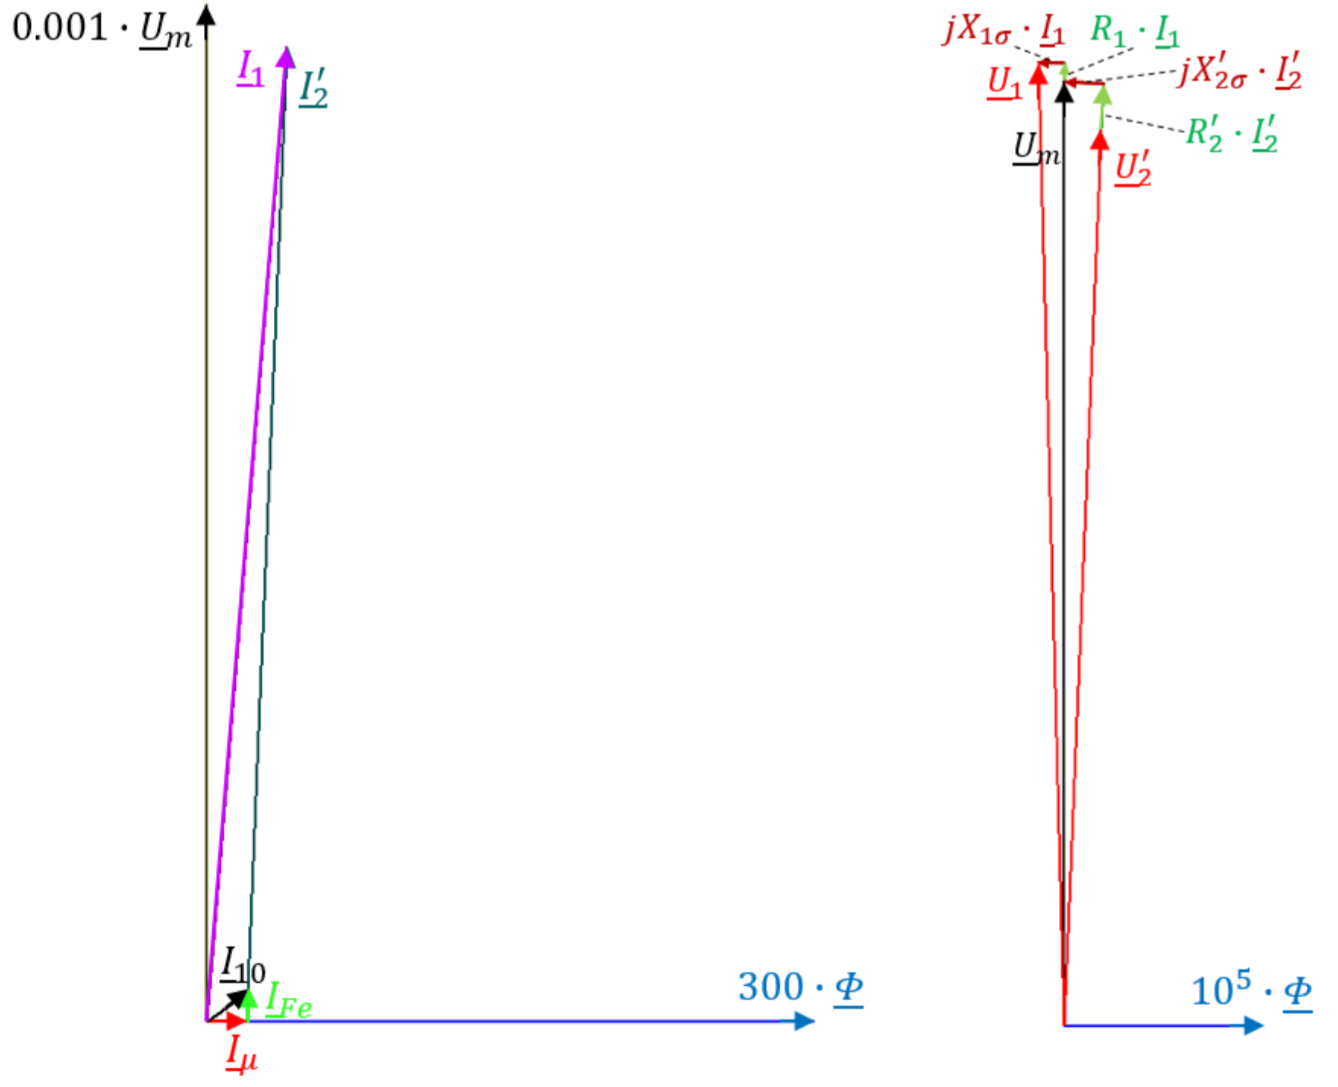
\includegraphics[width=0.9\textwidth]{bilder/a5.png}
\end{minipage}

\end{enumerate}


\begin{minipage}{0.4\textwidth}
Eigentlich ist der Fluss $\Phi_m$ reell und $U_m$ desshalb  $90^\circ$ verschoben (rein imaginär). Desshalb ist der Strom durch $R_{Fe}$ imaginär und durch $L_m$ reell!
\begin{enumerate}
	\itemsep0em 
	\item Alle Ströme und Spannungen gemäss Diagramm oben benamseln
	\item Maschengleichung 1: $\underline{U}_1 = \underline{U}_m+\underline{U}_{L1}+\underline{U}_{R1}$
	\item Maschengleichung 2: $\underline{U}_m=\underline{U}_{L2}'+\underline{U}_{R2}'+\underline{U}_2'$
	\item Knotengleichung 1:$\underline{I}_{10} = \underline{I}_\mu + \underline{I}_{Fe}$
	\item Knotengleichung 2:$\underline{I}_1 = \underline{I}_{10}
+ \underline{I}_{2}'$
	\item Zeigerdiagramm ausgehend von $\underline{U}_m$ auf der reellen Achse
	
\end{enumerate}
\end{minipage}
\begin{minipage}{0.59\textwidth}
\begin{align*}
	\underline{U}_1 &= j\cdot U_{10} = j\cdot 32kV\\
	\Phi_m&= \left(\frac{B\cdot A}{\sqrt{2}}\angle 0^\circ\right) = \left(\frac{1.8T\cdot 0.05m^2}{\sqrt{2}}\right) = 0.636Vs\\
	\hat{\underline{U}}_1 &= j\cdot \omega \cdot N_1\cdot B\cdot A_{Fe}\\
	I_{FE} &= j\cdot\frac{P_{FE}}{U_m} =j\cdot\frac{30kW}{32kV}=j\cdot 0,9375A\\
	I_\mu &= \frac{Q_u}{U_m} = \frac{40kVAr}{32kV} = 1.25A\\
	I_{10}&=I_{FE}+I_{\mu} = j\cdot 0.9375A+1,25A = (1.562A\angle 36.87^\circ)\\
	R_L &= \frac{P_N}{I_2^2} = \frac{10^6 VA}{(2500 A)^2}= 0.16\Omega \quad \textrm{Aus Nennlastbedingung}\\
	R_2' &= R_2\cdot  \left(\frac{N_1}{N_2}\right)^2=0.008\Omega\cdot\left(\frac{1600}{20}\right)^2= 51.2\Omega\\
	X_{\sigma 2}' &=X_{\sigma 2}\cdot \left(\frac{N_1}{N_2}\right)^2=0.007\Omega\cdot\left(\frac{1600}{20}\right)^2=  44.8\Omega\\
	I_2'&= \frac{\underline{U}_1}{\left(\frac{N_1}{N_2}\right)^2\cdot \left(R_L+ R_2+jX_{\sigma 2}\right) }\\
	& = \frac{j\cdot 32kV }{\left(\frac{1600}{20}\right)^2\cdot \left(0.16+0.008+j 0.007\right)\Omega} = 1.238+j\cdot 29.710\\
	I_1&=I_2'+I_\mu+I_{FE} = 1.238+j\cdot 29.710+1.25A+j\cdot 0.9375A\\
	&= (2.488+j\cdot 30.647)A
\end{align*}
\end{minipage}
\[
	\begin{array}{llll}
		U_1 &= R_1\cdot \underline{I}_1 + jX_{\sigma 1}\cdot  \underline{I}_1+\underline{U}_m &= (20 +j\cdot 30)\Omega\cdot (2.488+j\cdot 30.647)A+j\cdot 32'000V &= (-869+j\cdot 32786.6)V\\
		U_2 &= \underline{U}_m - R_2'\cdot \underline{I}_2' + jX_{\sigma 2}' \underline{I}_2' &= j\cdot 32'000V-(51.2 + j\cdot 44.8)\Omega \cdot (1.238+j\cdot 29,710)A&= (1267,622+j\cdot 30'423.386)V
	\end{array}	
\]

\subsection{Sternpunktverschiebung}
In einem Vierleiternetz $3x400V$ sind an $L1$ $60W$, an $L2$ $100W$, und an $L3$ $25W$ angeschlossen. Bestimmen sie die Verbraucherspannungen bei Neutralleiterunterbruch.\\
\begin{align*}
U_{1N} &= \frac{400V}{\sqrt{3}}\cdot e^{j\cdot 0^\circ} = 230.94V\cdot e^{j\cdot 0^\circ}\\
U_{2N} &= \frac{400V}{\sqrt{3}}\cdot e^{-j\cdot 120^\circ} = 230.94V\cdot e^{-j\cdot 120^\circ}\\
U_{3N} &= \frac{400V}{\sqrt{3}}\cdot e^{-j\cdot 240^\circ} = 230.94V\cdot e^{-j\cdot 240^\circ}\\
Y_1&=\frac{P_1}{U_{1N}}=\frac{60}{U_{1N}} = 1.125mS\\
Y_2&=\frac{P_2}{U_{2N}}=\frac{60}{U_{2N}} = 1.875mS\\
Y_3&=\frac{P_3}{U_{3N}}=\frac{60}{U_{3N}} = 0.4688mS\\
U_{nn'}&=-\frac{Y_1\cdot\underline{U_{1n}}+Y_2\cdot\underline{U_{2n}} Y_3\cdot\underline{U_{3n}}}{Y_1+Y_2+Y_3} = 81.141V\cdot e^{-j\cdot 92.2^\circ}\\
\underline{U_{1N'}} &= \underline{U_{1N}}+ \underline{U_{nn'}} =  247.71V\cdot e^{j\cdot 19.11^\circ}\\
\underline{U_{2N'}} &= \underline{U_{2N}}+ \underline{U_{nn'}} =  163.597V\cdot e^{-j\cdot 133.37 ^\circ}\\
\underline{U_{3N'}} &= \underline{U_{3N}}+ \underline{U_{nn'}} =  302.70V\cdot e^{j\cdot 111.79^\circ}\\
\end{align*}

\subsection{Symmetrische Belastung und Kompensation}
Ein Netzwerk mit 3x400V wird symmetrisch einem Verbraucher in Sternschaltung betrieben. Die Last ist ($R=20\Omega, L=48mH$).
\begin{align*}
I_1&= \frac{\underline{400V}}{\sqrt{3}\cdot \underline{Z}}= \frac{230.94V\angle0^\circ}{20+j\cdot100\cdot \pi \cdot 0.048H} = (9.22\angle-37.02^\circ )\\
I_2&= \frac{\underline{400V}}{\sqrt{3}\cdot \underline{Z}}= \frac{230.94V\angle -120^\circ}{20+j\cdot100\cdot \pi \cdot 0.048H} = (9.22\angle-157.02^\circ )\\
I_3&= \frac{\underline{400V}}{\sqrt{3}\cdot \underline{Z}}= \frac{230.94V\angle-240^\circ}{20+j\cdot100\cdot \pi \cdot 0.048H} = (9.22\angle 82.98^\circ )\\
S&=*\cdot \underline{U}\cdot \underline{I}^* = 3\cdot \frac{400}{\sqrt{3}}\cdot (9.22\angle-37.02^\circ ) = (6387.76\angle 37.01^\circ) VA = (5100.45+j\cdot3845.65)VA\\
P &= 5100.45W\\
Q &= 3845.65VAr\\
\cos(\varphi) = \cos(37.01^\circ) = 0.798
\end{align*}

Dieser Verbraucher soll nun auf einen $\cos(\varphi) = 0.92$ kompensiert werden. Berechnen sie das dazu nötige C.
\[
	C=\frac{(P_{str}\cdot \tan(\varphi_k)-P_{str}\cdot \tan(\varphi_k))}{\omega U^2} =\frac{(1700.15W\cdot \tan(\arccos(0.92))-1700.15W\cdot \tan(\arccos(0.798)))}{2\cdot\pi\cdot 50\cdot\left(\frac{400}{\sqrt{3}}\right)} = 33.4\mu F
\]
Der komplexe Verbraucher wird nun in Dreieckschaltung betrieben. Berechnen sie die Leistungen:
\[
	S_\Delta = 3\cdot S_Y = \frac{3\cdot \underline{U}\cdot \underline{U}^*}{\underline{Z}} = 15'301.35W+j\cdot 11'536.95VAr
\]


\newpage
\subsection{Drehstromtrafo}
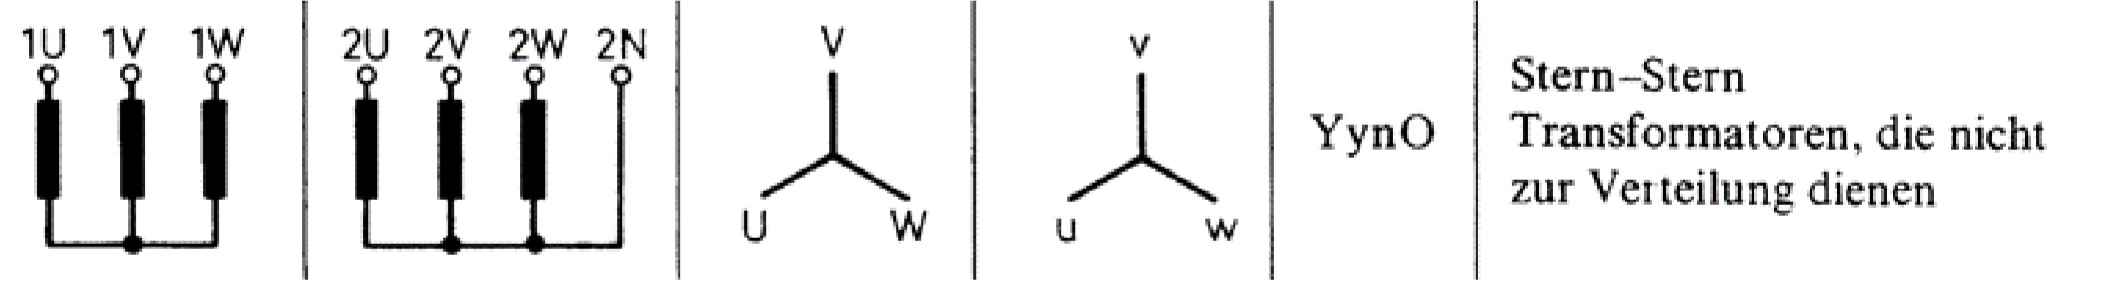
\includegraphics[width=0.99\textwidth]{bilder/a71.png}

\begin{minipage}{0.49\textwidth}
Von dem Trafo sind folgende Daten bekannt:
\begin{itemize}
\itemsep0em
\item Nennleistung $S_{1N} = 30MVA$
\item Primärnennspannung $ U_{1N} = 30kV / 50Hz$
\item Sekundärnennspannung $ U_{2N} = 10kV / 50Hz$ 
\item Windungszahlen je Strang $N_1 = 288$, $N_2 = 96$
\item Leerlaufstrom $I_{10} = 3.5A$
\item Leerlaufwirkleistung $P_{10} = 50.6kW$
\item Kurzschlussspannung $U_{1K} = 2700V$
\item Kurzschlusswirkleistung $P_{1K} = 152kW$
\end{itemize}
\end{minipage}
\begin{minipage}{0.49\textwidth}
\textbf{Einphasiges Ersatzschaltbild}

\adjustbox{width=0.8\textwidth}{\begin{circuitikz}[european]
	\draw (0,0) coordinate (In1) {} 
		to[short, *-, i=$\underline{I_1}$] ++(1,0)
		to[R, l=$R_1$] ++(2,0)
		to[L, l=$jX_{\sigma 1}$] ++(2,0)
		to[short, -*] ++(1,0) coordinate (middle1) {}
		to[short] ++(1,0)
		to[L, l=$jX'_{\sigma 2}$] ++(2,0)
		to[R, l=$R'_2$] ++(2,0)
		to[short, -* ,i<=$\underline{I_2}$] ++(1,0) coordinate(Out1);
	\draw (middle1) to[short, -*] ++(0,-1) coordinate (middle2) {};
	\draw (middle2) -- ++(-1,0) 
		to[R, l=$R_{Fe}$] ++(0,-2)
		to[short, -*] ++(1,0) coordinate(middle3)
		to[short, -*] ++(0,-1) coordinate(middle4);
	\draw (middle2) -- ++(1,0)
		to[L, l=$jX_h$] ++(0,-2)
		to[short] (middle3);
	\draw (middle4) to[short, -*] ++(-6,0) coordinate(In2);
	\draw (middle4) to[short, -*] ++(6,0) coordinate(Out2);
	\begin{scope}[
		shorten <=10pt,
		shorten >= 10pt,
		->
	]
		\draw (In1) -- (In2) node[midway, right] {$\underline{U_1}$};
		\draw (Out1) -- (Out2) node[midway, left] {$\underline{U'_2}$};
	\end{scope}
\end{circuitikz}}

\textbf{Einphasiges Ersatzschaltbild Leerlauf}

\adjustbox{width=0.6\textwidth}{\begin{circuitikz}[european]
	\draw (0,0) coordinate (In1) {} 
		to[short, *-, i=$\underline{I}_{10}$] ++(1,0)
		to[R, l=$R_1$] ++(2,0)
		to[L, l=$jX_{\sigma 1}$] ++(2,0)
		to[short, -*] ++(1,0) coordinate (middle1) {}
		to[short, -* ,i<=\mbox{$\underline{I}_2 = 0$}] ++(3,0) coordinate(Out1);
	\draw (middle1) to[short, -*] ++(0,-1) coordinate (middle2) {};
	\draw (middle2) 
		to[short, i_=$\underline{I}_{1Fe}$] ++(-1,0) 
		to[R, l=$R_{Fe}$] ++(0,-2)
		to[short, -*] ++(1,0) coordinate(middle3)
		to[short, -*] ++(0,-1) coordinate(middle4);
	\draw (middle2) 
		to[short, i=$\underline{I}_{1\mu}$] ++(1,0)
		to[L, l=$jX_h$] ++(0,-2)
		to[short] (middle3);
	\draw (middle4) to[short, -*] ++(-6,0) coordinate(In2);
	\draw (middle4) to[short, -*] ++(3,0) coordinate(Out2);
	\begin{scope}[
		shorten <=10pt,
		shorten >= 10pt,
		->
	]
		\draw (In1) -- (In2) node[midway, right] {$\underline{U}_{10}$};
		\draw (Out1) -- (Out2) node[midway, right] {$\underline{U}'_{20}$};
	\end{scope}
\end{circuitikz}}
\end{minipage}


\begin{enumerate}
\item Leerlaufberechnungen
\begin{align*}
	S_l &= \sqrt{3} \cdot U\cdot I = \sqrt{3} \cdot 30'000V\cdot 3.5A = 181.865kVA\\
	Q_L&= \sqrt{S_L^2-P_L^2} = \sqrt{(181.865kVA)^2-(50.6kW)^2} = 174.684kVAr\\
	&\textrm{Vernachlässigen von }R_1 \textrm{ und } X_{\sigma1}\\
	R_{FE}&=\frac{U_{10}^2}{P_{10}} = \frac{(30kV)^2}{50.6kW} = 17'786.8\Omega\\
	X_H &= \frac{U_{10}^2}{Q_L} = \frac{(30kV)^2}{174.684kVAr} = 5152.14\Omega\\
	L_H &= \frac{X_H}{\omega} = \frac{17.787k\Omega}{100\pi} = 16.399H
\end{align*}
\item Kurzschlussberechnungen
\begin{align*}
	I_{1N - 1\textrm{Phase}} &= \frac{30MVA}{3}\cdot \frac{\sqrt{3}}{30kVA} = 577.35A\\
	Z_K &= \frac{U_K}{\sqrt{3}}\cdot \frac{1}{I_{1N}} = \frac{2700}{\sqrt{3}\cdot 577.35A} = 2.7\Omega	\\
	P_K &= \sqrt{3}\cdot I_k^2\cdot R \Rightarrow R =\frac{P_k}{\sqrt{3}\cdot I_k^2} = \frac{152kW}{\sqrt{3}\cdot (577.35A)^2} = 0.152\Omega\\
	X_K &= \sqrt{Z^2 - R^2} = 2.6957\Omega\\
	Z &= (0.152+j\cdot 2.6957)\Omega
\end{align*}
\item Belastungsberechnungen
\begin{align*}
R_{2N}&= \frac{U^2_{2N}}{S_{2N}} = \frac{(10kV)^2}{30MVA} = 3.333\Omega \Rightarrow R'_2 = R_2\cdot  \left(\frac{288}{96}\right)^2 = 30\Omega\\ 
\underline{U'_2} &= \underline{U_1} - \underline{Z_K} \cdot \frac{\underline{U'_2}}{R'_2} = \frac{\underline{U_1}}{1+\frac{\underline{Z_K}}{R'_{2N}}} = \frac{30kV}{1+\frac{(0.152+j\cdot 2.6957)\Omega}{30\Omega}} = 29730.2V\angle -5.11^\circ\\
U_2 &= U'_2\cdot \frac{N_2}{N_1} = 29730.2V\angle -5.11^\circ \cdot \frac{96}{288} = 9910V\angle -5.11^\circ\\
P_{2N} &= \frac{U_2^2}{R_2} =\frac{(9910.06V)^2}{3.33333\Omega} = 29.462MVA\\
\eta &= \frac{P_2}{P_2+P_{10}+P_K} = \frac{29.462MVA}{29.462MVA+50.6KW+152kW} = 99.3\%
\end{align*}
\end{enumerate}






\subsection{Versorgungssysteme}
Gegeben ist die Vereinfachte Versorgungsschaltung bestehend aus:

\begin{itemize}
\item Netz $Q$ mit folgenden Kenndaten
\begin{itemize}
	\item Kurzschlussleistung $S_Q = 100MVA$
	\item Nennspannung $U_{NQ} = 10kV$
\end{itemize}
\item Der Transformator $T = Dyn5$ mit Kenndaten:
\begin{itemize}
	\item Übersetzung ü$ = \frac{10'000V}{400V}$
	\item Die Kurzschlussspannung $U_K\% = (0.77+j\cdot 3.5)\%$
	\item Betriebsleistung $S_B = 1MVA$
\end{itemize}
\item Die Leitung $L$
\begin{itemize}
	\item Länge $l = 100m$
	\item Imedanzbelag $Z_L' = (0.03+j\cdot 0.1)\Omega /km$
\end{itemize}
\item Zur Berechnung des Netzes sind folgende Annahmen zu treffen
\begin{itemize}
	\item Das Netz ist für $10\%$ Überspannung ausgelegt
	\item In Hoch und Mittelspannungsnetzen gilt: $\frac{R_Q}{X_Q}\approx 0.1$
\end{itemize}
\end{itemize}

\begin{figure}[h!]
    \begin{circuitikz}
      \draw (12,2)
      node[ocirc]{}
      to[R=$R_L$](10,2)
      to[L=$X_L$](8,2)
      node[ocirc]{}
      to[R=$R_{KT}$](6,2)
      to[L=$X_{KT}$](4,2)
      node[ocirc]{}
      to[R=$R_{Q}$](2,2)
      to[L=$X_{Q}$](0,2)
      to[V=$U_q{=\frac{1.1\cdot U_{NQ}}{\sqrt{3}}}$](0,0)
      to[short] (4,0)
      node[ocirc]{}
      to[short](8,0)
      node[ocirc]{}
      to[short] (12,0)
      node[ocirc]{}
      ;
    \end{circuitikz}
\end{figure}
\textbf{Berechnung der Netzimpedanz}\\
\begin{align*}
Z_Q &= \frac{1.1\cdot U_q}{\sqrt{3}\cdot I_k} = \frac{1.1\cdot U_{NQ}^2}{S_Q} = \frac{1.1\cdot 10'000^2}{100MVA}= 1.1\Omega\\
\frac{R_Q}{X_Q} &= 0.1 \Rightarrow Z_Q =\sqrt{R_Q^2+X_Q^2}  \Rightarrow X_Q = \frac{Z_Q}{1.005} = 1.0945\Omega\\
R_Q&= X_Q\cdot 0.1 = 0.10945\\	
Z_Q&= (0.10945 + j\cdot 1.0945)\Omega\\
U_{KVZ} &= \frac{U_K\%\cdot U_{TN2}}{100\%} = \frac{(0.77+j\cdot 3.5)\cdot 400V}{100\%} = (3.08+14j)V\\
S_N &= \sqrt{3} \cdot U_N\cdot I_N \Rightarrow \frac{S_N}{\sqrt{3}\cdot U_N} = \frac{1MVA}{\sqrt{3}\cdot 400V} = 1443.38A\\
Z_{KT} &= \frac{U_{KV2}}{\sqrt{3}\cdot I_N} =\frac{(3.08+14j)V}{\sqrt{3}\cdot 1443.38A} = (1.232+j\cdot 5.6)m\Omega\\
Z_L &= \frac{Z_L'}{l}\cdot L = (0.03+j\cdot 0.1) \cdot 0.1 = (3+j\cdot 10)m\Omega\\
R_K &= \frac{R_Q}{\left(\frac{N_1}{N_2}\right)^2} + R_{KT}+R_L = \frac{0.109\Omega}{\left(\frac{10'000}{400}\right)^2} + 1.232m\Omega+3m\Omega = 4.407m\Omega\\
X_K&= \frac{X_Q}{\left(\frac{N_1}{N_2}\right)^2} + x_{KT}+X_L = \frac{1094.5m\Omega	}{\left(\frac{10'000}{400}\right)^2} +5.6m\Omega+10m\Omega = 17.35m\Omega
\end{align*}

\newpage

\textbf{Berechnung des stationären Kurzschlusses}
\[
	I_K = \frac{\frac{1.1\cdot U_{NQ}}{\sqrt{3}}}{R+j\cdot X_K} = \frac{1.1\cdot 400V}{\sqrt{3}\cdot (4.407m\Omega + j\cdot 17.35m\Omega} = (14.19011\angle -75.75^\circ) kA 
\]
\[
	I_K(t) = \sqrt{2}\cdot 14.19kA\cdot \sin(2\pi 50Hz\cdot t-75.75^\circ)
\]

\textbf{Berechnung des transienten Kurzschlusses}\\
Da der Kurzschluss zu Beginn nicht rein Sinusförmig ist muss die DGL gelöst werden. Die partikuläre ist die stationäre Lösung und als solche bekannt. Die homogene Lösung muss berechnet werden.
\[\begin{array}{c}
R_K\cdot I_K + L_K\cdot \frac{dI_K}{dt} = 0\\
\frac{dI_K}{I_K} = -\frac{R_K}{L_K}\\
\ln(I_K) = -\frac{R_K}{I_K}\cdot t\\
I_K = B\cdot e^{-\frac{R_K}{I_K}\cdot t}\\
I_K(t) = B\cdot e^{-\frac{R_K}{I_K}\cdot t}+ \sqrt{2}\cdot 14.19kA\cdot \sin(2\pi 50Hz\cdot t-75.75^\circ)\\
\textrm{B aus Anfangsbedingungen}\quad I_K(0)=0\\
-B = \sqrt{2}\cdot 14.19kA \sin(-75.75^\circ) 
\end{array}\]



\newpage
\section{Riis\"a Tricks}
\input{idiotenseite/trigo/trigoInclude}
\input{idiotenseite/elektrotechnik/subsections/signalformen}

%%%%%%%%%%%%%%%%%%%%%%%%%%%%%%%%%%%%%%%%%%%%%%%%%%%%%%%%%%%%%%%%%%%%%%%%%%%%%%%%%%%%%%%%%%%%%%%%	
% \section{Komplexe Zahlen mit Taschenrecher - Texas Instruments}
% 	\begin{tabular}{p{4cm}p{10cm}}
% 	$\ldots \triangleright Rect $ 		& Umwandlung in Kartesische Darstellung \\
% 	$\ldots \triangleright Polar $ 		& Umwandlung in Polare Darstellung \\
% 	$conj(\ldots)$ 						& Konjugiert Komplex $\overline{z}$\\
% 	$abs(\ldots) $						& Betrag $|z|$\\
% 	$angle(\ldots) $					& Winkel $arg(z)$\\
% 	$imag(\ldots) $	s					& Imagin\"arteil $Im(z)$ \\
% 	$real(\ldots) $						& Realteil $Re(z)$ \\
% 	\end{tabular}

%%%%%%%%%%%%%%%%%%%%%%%%%%%%%%%%%%%%%%%%%%%%%%%%%%%%%%%%%%%%%%%%%%%%%%%%%%%%%%%%%%%%%%%%%%%%%%%%
%%%%%%%%%%%%%%%%%%%%%%%%%%%%%%%%%%%%%%%%%%%%%%%%%%%%%%%%%%%%%%%%%%%%%%%%%%%%%%%%%%%%%%%%%%%%%%%%


\end{document}